% Options for packages loaded elsewhere
\PassOptionsToPackage{unicode}{hyperref}
\PassOptionsToPackage{hyphens}{url}
\PassOptionsToPackage{dvipsnames,svgnames,x11names}{xcolor}
%
\documentclass[
  10pt,
  a4paper,
  twocolumn]{article}

\usepackage{amsmath,amssymb}
\usepackage{iftex}
\ifPDFTeX
  \usepackage[T1]{fontenc}
  \usepackage[utf8]{inputenc}
  \usepackage{textcomp} % provide euro and other symbols
\else % if luatex or xetex
  \usepackage{unicode-math}
  \defaultfontfeatures{Scale=MatchLowercase}
  \defaultfontfeatures[\rmfamily]{Ligatures=TeX,Scale=1}
\fi
\usepackage{lmodern}
\ifPDFTeX\else  
    % xetex/luatex font selection
\fi
% Use upquote if available, for straight quotes in verbatim environments
\IfFileExists{upquote.sty}{\usepackage{upquote}}{}
\IfFileExists{microtype.sty}{% use microtype if available
  \usepackage[]{microtype}
  \UseMicrotypeSet[protrusion]{basicmath} % disable protrusion for tt fonts
}{}
\makeatletter
\@ifundefined{KOMAClassName}{% if non-KOMA class
  \IfFileExists{parskip.sty}{%
    \usepackage{parskip}
  }{% else
    \setlength{\parindent}{0pt}
    \setlength{\parskip}{6pt plus 2pt minus 1pt}}
}{% if KOMA class
  \KOMAoptions{parskip=half}}
\makeatother
\usepackage{xcolor}
\usepackage[top=18mm,bottom=15mm,left=5mm,right=5mm]{geometry}
\ifLuaTeX
  \usepackage{luacolor}
  \usepackage[soul]{lua-ul}
\else
  \usepackage{soul}
  
\fi
\setlength{\emergencystretch}{3em} % prevent overfull lines
\setcounter{secnumdepth}{-\maxdimen} % remove section numbering
% Make \paragraph and \subparagraph free-standing
\makeatletter
\ifx\paragraph\undefined\else
  \let\oldparagraph\paragraph
  \renewcommand{\paragraph}{
    \@ifstar
      \xxxParagraphStar
      \xxxParagraphNoStar
  }
  \newcommand{\xxxParagraphStar}[1]{\oldparagraph*{#1}\mbox{}}
  \newcommand{\xxxParagraphNoStar}[1]{\oldparagraph{#1}\mbox{}}
\fi
\ifx\subparagraph\undefined\else
  \let\oldsubparagraph\subparagraph
  \renewcommand{\subparagraph}{
    \@ifstar
      \xxxSubParagraphStar
      \xxxSubParagraphNoStar
  }
  \newcommand{\xxxSubParagraphStar}[1]{\oldsubparagraph*{#1}\mbox{}}
  \newcommand{\xxxSubParagraphNoStar}[1]{\oldsubparagraph{#1}\mbox{}}
\fi
\makeatother

\usepackage{color}
\usepackage{fancyvrb}
\newcommand{\VerbBar}{|}
\newcommand{\VERB}{\Verb[commandchars=\\\{\}]}
\DefineVerbatimEnvironment{Highlighting}{Verbatim}{commandchars=\\\{\}}
% Add ',fontsize=\small' for more characters per line
\newenvironment{Shaded}{}{}
\newcommand{\AlertTok}[1]{\textcolor[rgb]{1.00,0.33,0.33}{\textbf{#1}}}
\newcommand{\AnnotationTok}[1]{\textcolor[rgb]{0.42,0.45,0.49}{#1}}
\newcommand{\AttributeTok}[1]{\textcolor[rgb]{0.84,0.23,0.29}{#1}}
\newcommand{\BaseNTok}[1]{\textcolor[rgb]{0.00,0.36,0.77}{#1}}
\newcommand{\BuiltInTok}[1]{\textcolor[rgb]{0.84,0.23,0.29}{#1}}
\newcommand{\CharTok}[1]{\textcolor[rgb]{0.01,0.18,0.38}{#1}}
\newcommand{\CommentTok}[1]{\textcolor[rgb]{0.42,0.45,0.49}{#1}}
\newcommand{\CommentVarTok}[1]{\textcolor[rgb]{0.42,0.45,0.49}{#1}}
\newcommand{\ConstantTok}[1]{\textcolor[rgb]{0.00,0.36,0.77}{#1}}
\newcommand{\ControlFlowTok}[1]{\textcolor[rgb]{0.84,0.23,0.29}{#1}}
\newcommand{\DataTypeTok}[1]{\textcolor[rgb]{0.84,0.23,0.29}{#1}}
\newcommand{\DecValTok}[1]{\textcolor[rgb]{0.00,0.36,0.77}{#1}}
\newcommand{\DocumentationTok}[1]{\textcolor[rgb]{0.42,0.45,0.49}{#1}}
\newcommand{\ErrorTok}[1]{\textcolor[rgb]{1.00,0.33,0.33}{\underline{#1}}}
\newcommand{\ExtensionTok}[1]{\textcolor[rgb]{0.84,0.23,0.29}{\textbf{#1}}}
\newcommand{\FloatTok}[1]{\textcolor[rgb]{0.00,0.36,0.77}{#1}}
\newcommand{\FunctionTok}[1]{\textcolor[rgb]{0.44,0.26,0.76}{#1}}
\newcommand{\ImportTok}[1]{\textcolor[rgb]{0.01,0.18,0.38}{#1}}
\newcommand{\InformationTok}[1]{\textcolor[rgb]{0.42,0.45,0.49}{#1}}
\newcommand{\KeywordTok}[1]{\textcolor[rgb]{0.84,0.23,0.29}{#1}}
\newcommand{\NormalTok}[1]{\textcolor[rgb]{0.14,0.16,0.18}{#1}}
\newcommand{\OperatorTok}[1]{\textcolor[rgb]{0.14,0.16,0.18}{#1}}
\newcommand{\OtherTok}[1]{\textcolor[rgb]{0.44,0.26,0.76}{#1}}
\newcommand{\PreprocessorTok}[1]{\textcolor[rgb]{0.84,0.23,0.29}{#1}}
\newcommand{\RegionMarkerTok}[1]{\textcolor[rgb]{0.42,0.45,0.49}{#1}}
\newcommand{\SpecialCharTok}[1]{\textcolor[rgb]{0.00,0.36,0.77}{#1}}
\newcommand{\SpecialStringTok}[1]{\textcolor[rgb]{0.01,0.18,0.38}{#1}}
\newcommand{\StringTok}[1]{\textcolor[rgb]{0.01,0.18,0.38}{#1}}
\newcommand{\VariableTok}[1]{\textcolor[rgb]{0.89,0.38,0.04}{#1}}
\newcommand{\VerbatimStringTok}[1]{\textcolor[rgb]{0.01,0.18,0.38}{#1}}
\newcommand{\WarningTok}[1]{\textcolor[rgb]{1.00,0.33,0.33}{#1}}

\providecommand{\tightlist}{%
  \setlength{\itemsep}{0pt}\setlength{\parskip}{0pt}}\usepackage{longtable,booktabs,array}
\usepackage{calc} % for calculating minipage widths
% Correct order of tables after \paragraph or \subparagraph
\usepackage{etoolbox}
\makeatletter
\patchcmd\longtable{\par}{\if@noskipsec\mbox{}\fi\par}{}{}
\makeatother
% Allow footnotes in longtable head/foot
\IfFileExists{footnotehyper.sty}{\usepackage{footnotehyper}}{\usepackage{footnote}}
\makesavenoteenv{longtable}
\usepackage{graphicx}
\makeatletter
\def\maxwidth{\ifdim\Gin@nat@width>\linewidth\linewidth\else\Gin@nat@width\fi}
\def\maxheight{\ifdim\Gin@nat@height>\textheight\textheight\else\Gin@nat@height\fi}
\makeatother
% Scale images if necessary, so that they will not overflow the page
% margins by default, and it is still possible to overwrite the defaults
% using explicit options in \includegraphics[width, height, ...]{}
\setkeys{Gin}{width=\maxwidth,height=\maxheight,keepaspectratio}
% Set default figure placement to htbp
\makeatletter
\def\fps@figure{htbp}
\makeatother

% this merely exists to fix the loading sequence (so 'floatrow' is loaded first before 'float')
\usepackage{floatrow}
\usepackage[datesep=.]{datetime2}
\DTMsetdatestyle{ddmmyyyy}
\usepackage{enumitem}
\setlist[description]{style=nextline,parsep=5mm}
\providecommand\phantomsection{}
\usepackage{multicol}
\usepackage{tikzscale}


\usepackage{xfrac}


\DeclareRobustCommand{\textHighlight}[1]{\tikz[baseline]{\node[anchor=base,fill=Gray!10, rounded corners=5pt, draw, densely dotted] {\bfseries{#1}};}}

\makeatletter
\newcommand{\shorteq}{\mathrel{\mkern0.2mu\mathpalette\shorteq@\relax\mkern0.2mu}}
\newcommand{\shorteq@}[2]{\scalebox{0.5}[1]{$\m@th#1=$}}

\newcommand{\longeq}[1]{\mathrel{\mathpalette\longeq@{#1}}}
\newcommand{\longeq@}[2]{%
  \begingroup
  \sbox\z@{$\m@th#1=$}%
  \ifdim#2<\wd\z@
    \resizebox{#2}{\height}{\box\z@}%
  \else
    \ifdim#2<3\wd\z@
      \hbox to #2{$\m@th#1=\hss=\hss=\hss=$}%
    \else
      \hbox to #2{$\m@th#1=\cleaders\hbox to 0.2\wd\z@{\hss$#1=$\hss}\hfil=$}%
    \fi
  \fi
  \endgroup
}
\makeatother
\makeatletter
\@ifpackageloaded{tcolorbox}{}{\usepackage[skins,breakable]{tcolorbox}}
\@ifpackageloaded{fontawesome5}{}{\usepackage{fontawesome5}}
\definecolor{quarto-callout-color}{HTML}{909090}
\definecolor{quarto-callout-note-color}{HTML}{0758E5}
\definecolor{quarto-callout-important-color}{HTML}{CC1914}
\definecolor{quarto-callout-warning-color}{HTML}{EB9113}
\definecolor{quarto-callout-tip-color}{HTML}{00A047}
\definecolor{quarto-callout-caution-color}{HTML}{FC5300}
\definecolor{quarto-callout-color-frame}{HTML}{acacac}
\definecolor{quarto-callout-note-color-frame}{HTML}{4582ec}
\definecolor{quarto-callout-important-color-frame}{HTML}{d9534f}
\definecolor{quarto-callout-warning-color-frame}{HTML}{f0ad4e}
\definecolor{quarto-callout-tip-color-frame}{HTML}{02b875}
\definecolor{quarto-callout-caution-color-frame}{HTML}{fd7e14}
\makeatother
\makeatletter
\@ifpackageloaded{caption}{}{\usepackage{caption}}
\AtBeginDocument{%
\ifdefined\contentsname
  \renewcommand*\contentsname{Inhaltsverzeichnis}
\else
  \newcommand\contentsname{Inhaltsverzeichnis}
\fi
\ifdefined\listfigurename
  \renewcommand*\listfigurename{Abbildungsverzeichnis}
\else
  \newcommand\listfigurename{Abbildungsverzeichnis}
\fi
\ifdefined\listtablename
  \renewcommand*\listtablename{Tabellenverzeichnis}
\else
  \newcommand\listtablename{Tabellenverzeichnis}
\fi
\ifdefined\figurename
  \renewcommand*\figurename{Abbildung}
\else
  \newcommand\figurename{Abbildung}
\fi
\ifdefined\tablename
  \renewcommand*\tablename{Tabelle}
\else
  \newcommand\tablename{Tabelle}
\fi
}
\@ifpackageloaded{float}{}{\usepackage{float}}
\floatstyle{ruled}
\@ifundefined{c@chapter}{\newfloat{codelisting}{h}{lop}}{\newfloat{codelisting}{h}{lop}[chapter]}
\floatname{codelisting}{Listing}
\newcommand*\listoflistings{\listof{codelisting}{Listingverzeichnis}}
\makeatother
\makeatletter
\makeatother
\makeatletter
\@ifpackageloaded{caption}{}{\usepackage{caption}}
\@ifpackageloaded{subcaption}{}{\usepackage{subcaption}}
\makeatother
\makeatletter
\@ifpackageloaded{tcolorbox}{}{\usepackage[skins,breakable]{tcolorbox}}
\makeatother
\makeatletter
\@ifundefined{shadecolor}{\definecolor{shadecolor}{rgb}{.97, .97, .97}}{}
\makeatother
\makeatletter
\@ifundefined{codebgcolor}{\definecolor{codebgcolor}{HTML}{f7f7f7}}{}
\makeatother
\makeatletter
\ifdefined\Shaded\renewenvironment{Shaded}{\begin{tcolorbox}[frame hidden, enhanced, sharp corners, colback={codebgcolor}, breakable, boxrule=0pt]}{\end{tcolorbox}}\fi
\makeatother
\makeatletter
\@ifpackageloaded{tikz}{}{\usepackage{tikz}}
\makeatother
        \newcommand*\circled[1]{\tikz[baseline=(char.base)]{
          \node[shape=circle,draw,inner sep=1pt] (char) {{\scriptsize#1}};}}  
                  
\ifLuaTeX
\usepackage[bidi=basic]{babel}
\else
\usepackage[bidi=default]{babel}
\fi
\babelprovide[main,import]{nswissgerman}
% get rid of language-specific shorthands (see #6817):
\let\LanguageShortHands\languageshorthands
\def\languageshorthands#1{}
\ifLuaTeX
  \usepackage{selnolig}  % disable illegal ligatures
\fi
\usepackage{bookmark}

\IfFileExists{xurl.sty}{\usepackage{xurl}}{} % add URL line breaks if available
\urlstyle{same} % disable monospaced font for URLs
\hypersetup{
  pdftitle={Advanced System Design},
  pdfauthor={Joel von Rotz},
  pdflang={de-CH},
  colorlinks=true,
  linkcolor={blue},
  filecolor={Maroon},
  citecolor={Blue},
  urlcolor={Blue},
  pdfcreator={LaTeX via pandoc}}


% [GENERAL PACKAGES] ------------------------------------------------------------------- %
% includes some neato math environments, symbols and stuff
\usepackage{amssymb, amsmath}

% correctly encodes the formatting of the text files (since we live in the future of UTF8)
\usepackage[utf8]{inputenc} 

% Used for the page counter in the footer to see the amount of pages 
\usepackage{lastpage} 

% Mostly used for the titlepage. Compared to the 'twocolumn' mode, multicols allows for
% more flexible changing (without inserting newpage between column mode changes)
\usepackage{multicol}
\setlength\columnsep{20pt}

% Package for enabling colors (colorful output)
\usepackage[dvipsnames]{xcolor}
\definecolor{colorAccent}{HTML}{124E82}

% Icons - http://mirrors.ctan.org/fonts/fontawesome5/doc/fontawesome5.pdf
% This one is neat, when you want to add some icons
\usepackage{fontawesome5}

% Depending on the type of document, mostly summaries, I remove the spacing Display-styled Equations insert, since it's a waste of space.
\usepackage[nodisplayskipstretch]{setspace}

% [FONT CONFIGURATION] ----------------------------------------------------------------- %
% change the fonts here (depending which latex engine is used, this might need to be
% removed)

\usepackage{AlegreyaSans}
\usepackage{cmbright}
\usepackage[scaled=0.95]{inconsolata}

% \usepackage{AlegreyaSans}
% \usepackage{cmbright}
% \usepackage[scaled=0.95]{inconsolata} % for code blocks

% [TIKZ CONFIGURATION] ----------------------------------------------------------------- %
% Tikz is really good at creating nice looking and clean drawings, diagramms, etc. 
\usepackage{tikz}
\usetikzlibrary{shapes,arrows,arrows.meta,matrix,decorations.pathmorphing}
%\newcommand*\circled[1]{\tikz[baseline=(char.base)]{
%            \node[shape=circle,draw,inner sep=2pt] (char) {#1};}}

% TIP: use 'TikzEdt' (http://www.tikzedt.org/) to preview the drawings.

% [HEADING/SECTION STYLE CONFIGURATION] ------------------------------------------------ %
% 'sectsty' is used for minor adjustments and is used to apply the bold sans serif style
% to all sections (sec, subsec, subsubsec, ...)
\usepackage{sectsty}
\allsectionsfont{\normalfont\bfseries\sffamily}

% 'titlesec' is used to customize the numbered and unnumbered sections styles (but can
% also be used for the other section types).
% 'xhfill' is used to add a ruler, centered to the text.
\usepackage{xhfill}
\usepackage[explicit]{titlesec}

\makeatletter
\newcommand \Cdotfill {\leavevmode\cleaders\hb@xt@.25em{\hss$\cdot$\hss}\hfill\kern\z@}
\makeatother

% NUMBERED - SECTIION
\titleformat
  {\section} % {⟨command⟩}
  [hang] % [⟨shape⟩]
  {\normalfont\LARGE\bfseries\filright\sffamily} % {⟨format⟩}
  {\thesection} % {⟨label⟩}
  {3mm} % {⟨sep⟩}
  {%
    \color{colorAccent}{#1\hspace{2mm}\xrfill[0.6ex]{1pt}}
  } % {⟨before-code⟩}

\titlespacing*{\section} % ⟨command⟩
  {0em} % ⟨left⟩
  {12pt} % ⟨before-sep⟩
  {6pt} % ⟨after-sep⟩

% NUMBERLESS - SECTION
\titleformat
  {name=\section,numberless} % {⟨command⟩}
  [hang] % [⟨shape⟩]
  {\normalfont\LARGE\bfseries\filright\sffamily} % {⟨format⟩}
  {} % {⟨label⟩}
  {0mm} % {⟨sep⟩}
  {%
    \color{colorAccent}{#1\hspace{2mm}}\xrfill[0.6ex]{1.2pt}[colorAccent]
  }% {⟨before-code⟩}

% NUMBERED - SUBSECTION
\titleformat{\subsection} % {⟨command⟩}
  [hang] % [⟨shape⟩]
  {\normalfont\Large\bfseries\filright\sffamily} % {⟨format⟩}
  {\thesection} % {⟨label⟩}
  {2mm} % {⟨sep⟩}
  {%
    {#1\hspace{1mm}\color{colorAccent}{\Cdotfill}}%
  } % {⟨before-code⟩}

% NUMBERLESS - SUBSECTION
\titleformat{name=\subsection,numberless} % {⟨command⟩}
  [hang] % [⟨shape⟩]
  {\normalfont\Large\bfseries\filright\sffamily} % {⟨format⟩}
  {} % {⟨label⟩}
  {0mm} % {⟨sep⟩}
  {%
    {#1\hspace{1mm}\color{colorAccent}{\Cdotfill}}%
  }% {⟨before-code⟩}

\titlespacing*{\subsection} % <command>
  {0em} % <left>
  {.5em} % <before-sep>
  {.4em} % <after-sep>

% NUMBERED - SUBSUBSECTION
\titleformat{\subsubsection} % {⟨command⟩}
  [hang] % [⟨shape⟩]
  {\normalfont\large\bfseries\sffamily} % {⟨format⟩}
  {\thesection} % {⟨label⟩}
  {2mm} % {⟨sep⟩}
  {
    #1%
  } % {⟨before-code⟩}

% NUMBERLESS - SUBSUBSECTION
\titleformat{name=\subsubsection,numberless} % {⟨command⟩}
  [hang] % [⟨shape⟩]
  {\normalfont\large\bfseries\sffamily} % {⟨format⟩}
  {} % {⟨label⟩}
  {0mm} % {⟨sep⟩}
  {%
    #1%
  }% {⟨before-code⟩}

% [HEADER & FOOTER CONFIGURATION] ------------------------------------------------------ %
% Most configuration is done through the quarto project yaml file (aka. '_quarto.yml').
% 
% Inside '_quarto.yml' use following structure. If one is not used, uncomment it:
%
%  fancyhdr:
%    header:
%      right: "text"
%      center: "text"
%      left: "text"
%    footer:
%      right: "text"
%      center: "text"
%      left: "text"
\usepackage{fancyhdr}
\pagestyle{fancy}

% This adds the section number to the rightmark command, which is usually used for the
% header/footer
\renewcommand{\sectionmark}[1]{\markright{#1}}
\renewcommand{\subsectionmark}[1]{}

% Adds a rules to the header and footer
\renewcommand{\headrulewidth}{1pt}
\renewcommand{\footrulewidth}{1pt}

\fancyhf{} % clear all header and footer fields
% header
\fancyhead[R]{\sffamily Advanced System Design - Zusammenfassung}


\fancyhead[L]{\sffamily HSLU T\&A}

% header
\fancyfoot[R]{\sffamily ASYD}

\fancyfoot[C]{\sffamily \thepage~/ \pageref{LastPage}}

\fancyfoot[L]{\sffamily \DTMtoday}

% [CONDITIONS ENVIRONMENT] ------------------------------------------------------------- %
% introduces conditions environment to create nice equation parameter description
% note: the first column is already in math mode, so no $ are required.
%
% \begin{conditions}
%   A & Description about A \\
%   B & Description about B \\
%   C & Description about C
% \begin{conditions}
%
\usepackage{array}
\newenvironment{conditions}
  {\par\vspace{\abovedisplayskip}\noindent\begin{tabular}{>{$}l<{$} @{${}:{}$} l}}
  {\end{tabular}\par\vspace{\belowdisplayskip}}

\usepackage{tabularx}
\newenvironment{conditions*}
  {\par\vspace{\abovedisplayskip}\noindent
   \tabularx{\columnwidth}{>{$}l<{$} @{${}:{}$} >{\raggedright\arraybackslash}X}}
  {\endtabularx\par\vspace{\belowdisplayskip}}

% [FANCY VERBATIM] --------------------------------------------------------------------- %
% in combination with the file 'before-content.tex' inside the 'config' folder, the
% packages 'fancyvbr', 'fvextra' and 'floatrow' are used to restyle the implemented
% Verbatim/Codeblock styles to make it (personally) nicer looking and include breaklines +
% symbols
\usepackage{fancyvrb}
\definecolor{codeRuleColor}{HTML}{1a1e2e}
\definecolor{codeLineNumberColor}{HTML}{84858a}

% This reconfigures the code block to make a little nicer to look at.
% The following renewcommand 
\renewcommand{\theFancyVerbLine}{%
  \textcolor{codeLineNumberColor}{\ttfamily\scriptsize
  \arabic{FancyVerbLine}}}

\usepackage{fvextra}
\DefineVerbatimEnvironment{Highlighting} % Its new name
  {Verbatim} % Based on this environment
  {
    breaklines,
    breaksymbolleft={\textcolor{gray}{\scriptsize\ensuremath\hookrightarrow}},
    commandchars=\\\{\},
    rulecolor=\color{codeRuleColor},
    xleftmargin=1mm
  }


\DeclareFloatStyle{MyListingStyle}
  {
    style=plaintop,
    captionskip=1pt
  }

% [MISC] ------------------------------------------------------------------------------- %


% -------------------------------------------------------------------------------------- %
\title{Advanced System Design}
\usepackage{etoolbox}
\makeatletter
\providecommand{\subtitle}[1]{% add subtitle to \maketitle
  \apptocmd{\@title}{\par {\large #1 \par}}{}{}
}
\makeatother
\subtitle{Zusammenfassung}
\author{Joel von Rotz}
\date{}

\begin{document}

  \raggedcolumns
  
\makeatletter
\begin{center}
  \vspace*{0.5cm}
  \textbf{\textsf{\Huge Advanced System Design}}\\
  \vspace{0.1cm}
  \textsf{\textit{\large Zusammenfassung}}\\
  \vspace{0.5cm}
  \textsf{\large Joel von
Rotz \hspace{0.3cm}\textbf{/}\hspace{0.3cm}\mbox{\large \faGithub\space \href{https://github.com/joelvonrotz/BSc-electrical-engineering/tree/main/semester\%206/advanced\%20system\%20design}{Quelldateien}}}
\end{center}
\makeatother
\normalfont


% Workaround to fix some subtle things, such as caption style for code blcocks.

% changes the preset style
\floatsetup[codelisting]{style=MyListingStyle}

% include the current section number into the different caption types
\numberwithin{equation}{section}
\numberwithin{codelisting}{section}
\numberwithin{figure}{section}
\numberwithin{table}{section}

% if no code blocks are used, 'Shaded' doesn't exist!
\ifdefined\Shaded
  % redefine the Shaded environment to make the codeblock more bearable to 
  \renewenvironment{Shaded}
    {\begin{tcolorbox}[
      rounded corners,
      colback={codebgcolor},
      colframe={codebgcolor},
      enhanced,
      boxrule=0mm,
      borderline={1pt}{0pt}{gray,dotted},
      left=0mm,
      breakable,
      %title after break={Theorem \themytheorem\ Continued}, % works, but not great
      overlay first={%
          \draw[thick,gray,line width=0.5pt,decoration={zigzag,segment length=4mm, amplitude=2mm/(2*sqrt(2))},decorate]
            (frame.south west) -- (frame.south east);
      },
      overlay middle={%
          \draw[thick,gray,line width=0.5pt,decoration={zigzag,segment length=4mm, amplitude=2mm/(2*sqrt(2))},decorate]
            (frame.south west) -- (frame.south east);
          \draw[thick,gray,line width=0.5pt,decoration={zigzag,segment length=4mm, amplitude=2mm/(2*sqrt(2))},decorate]
            (frame.north west) -- (frame.north east);
      },
      overlay last={%
          \draw[thick,gray,line width=0.5pt,decoration={zigzag,segment length=4mm, amplitude=2mm/(2*sqrt(2))},decorate]
            (frame.north west) -- (frame.north east);
      }
      ]}
    {\end{tcolorbox}}
\fi

\renewcommand*\contentsname{Inhaltsverzeichnis}
{
\hypersetup{linkcolor=}
\setcounter{tocdepth}{3}
\tableofcontents
}
\newpage

\section{Crypto}\label{crypto}


\includegraphics[width=7cm,height=\textheight]{images/crypto_meme.jpg}

\begin{tcolorbox}[enhanced jigsaw, toprule=.15mm, opacityback=0, colbacktitle=quarto-callout-note-color!10!white, breakable, colframe=quarto-callout-note-color-frame, title=\textcolor{quarto-callout-note-color}{\faInfo}\hspace{0.5em}{Hinweis}, left=2mm, arc=.35mm, toptitle=1mm, bottomrule=.15mm, rightrule=.15mm, titlerule=0mm, bottomtitle=1mm, leftrule=.75mm, opacitybacktitle=0.6, coltitle=black, colback=white]

Wenn Daten Sequenzen in Blöcke geteilt werden (z.B. 64-Bit), dann wird
davon ausgegangen, dass bei unvollständigen Blöcken die restlichen Bits
mit z.B. \texttt{0} augefüllt werden.

\end{tcolorbox}

\subsection{Cesar Cipher / Substitution
Cipher}\label{cesar-cipher-substitution-cipher}

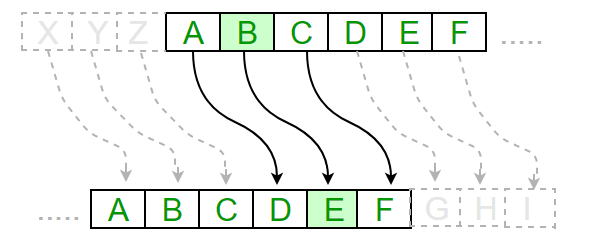
\includegraphics{images/crypto/ceaserCipher.png}

Buchstaben werden um \(x\) Positionen verschoben (z.B.
\texttt{A}\(\overset{+2}{\rightarrow}\)\texttt{C}). Nachteil ist, dass
die Entschlüsselung sehr einfach ist.

\subsection{\texorpdfstring{Enigma Maschine
\href{https://www.youtube.com/watch?v=ybkkiGtJmkM}{\color{BrickRed}\faYoutube}}{Enigma Maschine }}\label{enigma-maschine}

Die Enigma Maschine ist ein komplexes Ent- \& Verschlüsselungs System,
welches während den Weltkriegen von den Nazis hauptsächlich verwendet
wurde (und durch Alan Turing geknackt).

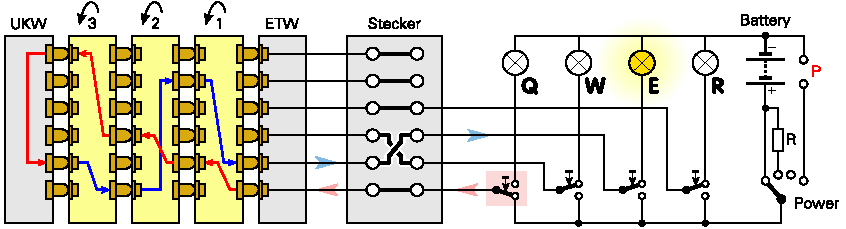
\includegraphics{images/crypto/enigma.pdf}

Nachjedem Tastendruck leuchtet ein Buchstabe auf und die Rotoren drehen
sich, damit der nächste gleiche Tastendruck nicht den gleichen Buchstabe
ergibt. Mit den Steckern können die Buchstaben umkonfiguriert werden
(bei Doppelstecker wird z.B. \(A\rightarrow B\) \& \(B\rightarrow A\)
und dadurch halbiert sich die Möglichkeiten zu 13).

\subsection{Stream \& Block Cipher}\label{stream-block-cipher}

\begin{center}
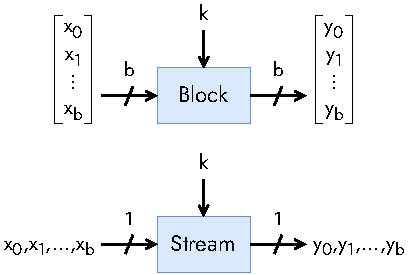
\includegraphics{images/crypto/block_stream_cipher.pdf}
\end{center}

\subsection{Konfusion}\label{konfusion}

Konfusion ist eine Verschlüsselungsoperation, bei der die
\textbf{Beziehung zwischen Key und Ciphertext verschleiert} wird. Ein
gängiges Element zur Erzielung von Konfusion ist heute die Substitution.

Konfusion erhöht die Mehrdeutigkeit des Ciphertextes und wird sowohl von
Block- als auch von Stream-Ciphern verwendet.

\subsection{Diffusion}\label{diffusion}

Diffusion ist eine Verschlüsselungsoperation, bei der der Einfluss eines
Klartextsymbols auf viele Ciphertext-Symbole verteilt wird, um die
statistischen Eigenschaften des Klartextes zu verbergen.

\subsection{\texorpdfstring{Feistel Network
\href{https://www.youtube.com/watch?v=FGhj3CGxl8I}{\color{BrickRed}\faYoutube}}{Feistel Network }}\label{feistel-network}

Ein Feistel Netzwerk wird zum Ver- und Entschlüsseln von Datenpaketen
verwendet. Folgend ist ein symmetrisches Feistel Netzwerk
\(\rightarrow\) Datenblock wird halbiert (64-Bit \(\rightarrow\) 2
\(\times\) 32-Bit). Eine Runde entspricht:

\[
\begin{split}
  L_n &= R_{n-1}\\
  R_n &= f(L_{n-1},k_n)
\end{split}
\]

\begin{center}
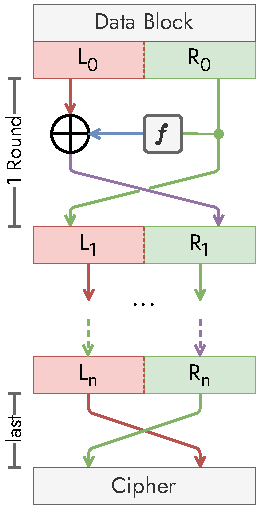
\includegraphics[width=4cm,height=\textheight]{images/crypto/feistel_network.pdf}
\end{center}

Funktion \(f\) ist \textbf{wichtig}. Wenn diese sicher gegen Attacken
ist, dann wird das Feistel Netzwerk mit jeder Runde und Key-Segment
sicherer!

\begin{tcolorbox}[enhanced jigsaw, toprule=.15mm, opacityback=0, colbacktitle=quarto-callout-important-color!10!white, breakable, colframe=quarto-callout-important-color-frame, title=\textcolor{quarto-callout-important-color}{\faExclamation}\hspace{0.5em}{Ver- \& Entschlüsseln}, left=2mm, arc=.35mm, toptitle=1mm, bottomrule=.15mm, rightrule=.15mm, titlerule=0mm, bottomtitle=1mm, leftrule=.75mm, opacitybacktitle=0.6, coltitle=black, colback=white]

Verschlüsselte Informationen können mit dem genau gleichen Ablauf wieder
entschlüsselt werden.

\end{tcolorbox}

\subsection{\texorpdfstring{DES
\href{https://www.youtube.com/watch?v=3BZRBfhpIb0}{\color{BrickRed}\faYoutube}}{DES }}\label{des}

\textbf{D}ata \textbf{E}ncryption \textbf{S}tandard ist ein Cipher, der
64 Bit lange Blöcke mit einem 56 Bit langen Schlüssel verschlüsselt.

\begin{center}
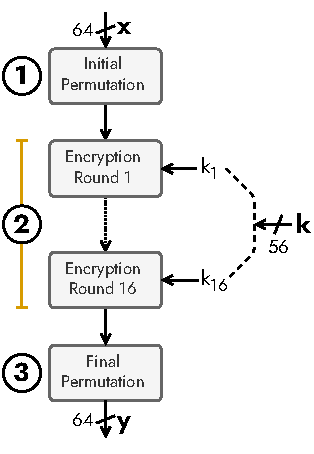
\includegraphics{images/crypto/des.pdf}
\end{center}

\begin{enumerate}
\def\labelenumi{\arabic{enumi}.}
\tightlist
\item
  Data \(x\) wird mit einer \emph{Initial Permutation} transponiert
  (\textbf{Diffusion})
\item
  Diffusierte Data wird wird im Feistel Netzwerk \textbf{16×}
  verschlüsselt
\item
  Die verschlüsselte Data wird mit einer \emph{Final Permutation} wieder
  transponiert (\textbf{Diffusion})
\end{enumerate}

\begin{center}
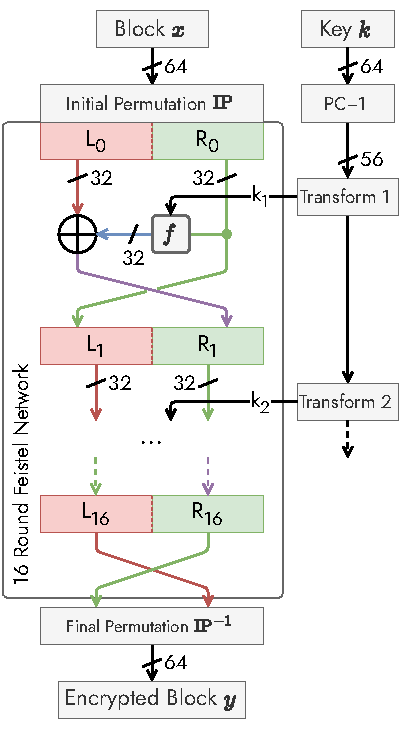
\includegraphics{images/crypto/des_detailed.pdf}
\end{center}

\subsubsection{Initial \& Final
Permutation}\label{initial-final-permutation}

Vor und nach dem Feistel Netzwerk werden die Blöcke bitweise permutiert,
also wie kreuzverdrahtet (Enigma Steckerbrett) \(\rightarrow\) Bit
\textbf{Diffusion}

\begin{tcolorbox}[enhanced jigsaw, toprule=.15mm, opacityback=0, colbacktitle=quarto-callout-note-color!10!white, breakable, colframe=quarto-callout-note-color-frame, title=\textcolor{quarto-callout-note-color}{\faInfo}\hspace{0.5em}{Hinweis}, left=2mm, arc=.35mm, toptitle=1mm, bottomrule=.15mm, rightrule=.15mm, titlerule=0mm, bottomtitle=1mm, leftrule=.75mm, opacitybacktitle=0.6, coltitle=black, colback=white]

Diese Permutationen sind in Hardware einfacher implementierbar als in
der Software.

\end{tcolorbox}

\subsubsection{\texorpdfstring{\(f\)-Funktion}{f-Funktion}}\label{f-funktion}

Die \(f\)-Funktion vom DES ist das Herz des Algorithmus.

\begin{center}
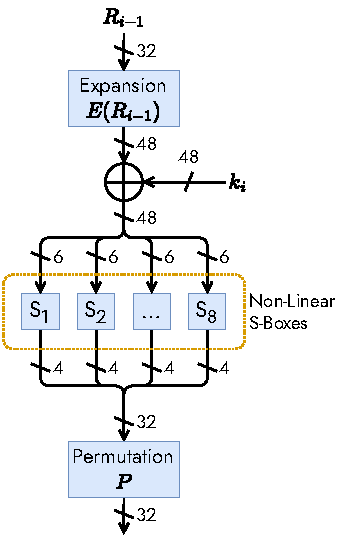
\includegraphics{images/crypto/des_ffunction.pdf}
\end{center}

\begin{enumerate}
\def\labelenumi{\arabic{enumi}.}
\tightlist
\item
  Das Datenbyte \(R_{i-1}\) wird mit expandiert (Doppelzuweisung) um auf
  48 Bit zu kommen\ldots{}
\item
  \ldots danach wird dies mit dem Key ver\textbf{xor}t und\ldots{}
\item
  \ldots mit der jeweiligen Substitutationsbox (LUT) \(S_x\)
  verarbeitet.
\item
  Schlussendlich
\end{enumerate}

\subsubsection{\texorpdfstring{Expansion
\(E\)}{Expansion E}}\label{expansion-e}

Expansion \(E\) ist eine spezielle Permutationsfunktion. Die Expansion
wird von 32-Bits zu 48-Bits \emph{expandiert}.

\begin{center}
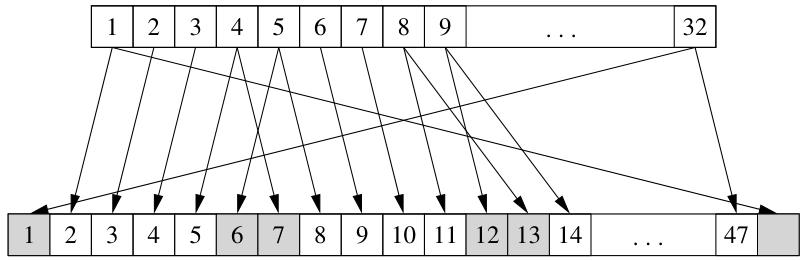
\includegraphics[width=6cm,height=\textheight]{images/crypto/expansion_function.png}
\end{center}

\begin{tcolorbox}[enhanced jigsaw, toprule=.15mm, opacityback=0, colbacktitle=quarto-callout-important-color!10!white, breakable, colframe=quarto-callout-important-color-frame, title=\textcolor{quarto-callout-important-color}{\faExclamation}\hspace{0.5em}{Wichtig}, left=2mm, arc=.35mm, toptitle=1mm, bottomrule=.15mm, rightrule=.15mm, titlerule=0mm, bottomtitle=1mm, leftrule=.75mm, opacitybacktitle=0.6, coltitle=black, colback=white]

16-Bit der 32 Input-Bits kommen doppelt vor. \textbf{ABER} ein Input-Bit
kommt \textbf{nicht} zweimal vor im selben 6-Bit Block \(\rightarrow\)
Diffusion wird verbessert, da gewisse Input-Bits zweimal vorkommen.

\end{tcolorbox}

\subsubsection{\texorpdfstring{Key Scheduling Transform
\(X\)}{Key Scheduling Transform X}}\label{key-scheduling-transform-x}

Der \emph{Key Scheduler} generiert 16 Subkeys \(k_i\) vom Hauptkey
\(k\).

\begin{enumerate}
\def\labelenumi{\arabic{enumi}.}
\tightlist
\item
  Der Key wird in \(PC-1\) auf 56-Bits gekürzt. Die \emph{Parity} Bits
  8, 16, 24, 32, 40, 48, 56 \& 64 werden entfernt \(\rightarrow\)
  sinnlose Bits
\end{enumerate}

\begin{center}
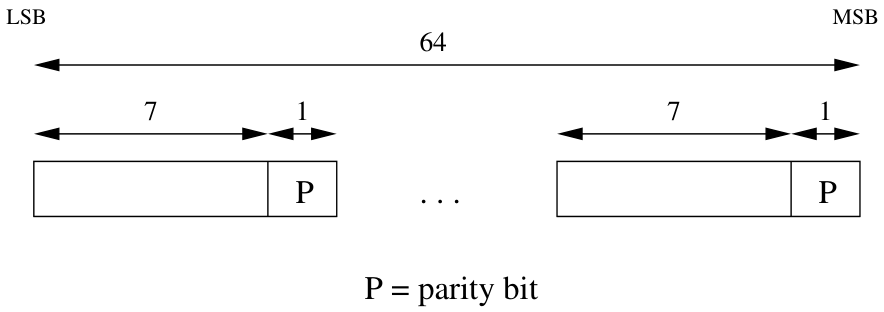
\includegraphics[width=6cm,height=\textheight]{images/crypto/initial_key_permutation.png}
\end{center}

\begin{enumerate}
\def\labelenumi{\arabic{enumi}.}
\setcounter{enumi}{1}
\item
  In Runden \(i=1,2,9,16\) wird \(C_n\) \textbf{ein} Bit nach links
  geshiftet, ansonsten \textbf{zwei} Bits.
\item
  In \(PC-2\) werden erneut 8 Bits verworfen \(\rightarrow\) 48 Bit
  Subkey \(k_i\)
\end{enumerate}

\begin{center}
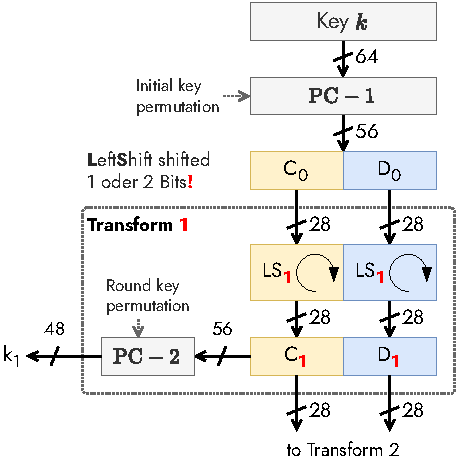
\includegraphics{images/crypto/keyscheduler.pdf}
\end{center}

\subsubsection{Das Coole}\label{das-coole}

Der Cipher kann mit dem gleichen System wieder entschlüsselt werden. DES
verwendet als Grundelement das Feistel Netzwerk, welches diese
Eigenschaft hat.

\subsubsection{Das Problem}\label{das-problem}

DES ist wegen der kleinen 56 Bit Key nicht sicher (Fall: 1993 \& 2008
Brute Force), was ja auch nid so doll is'. Ein Ansatz dafür ist den Key
auf 112 Bits zu erweitern durch \textbf{triple DES}
(\(\text{DES}(k_1)+\text{DES}^{-1}(k_2)+\text{DES}(k_2)\)).

\subsection{\texorpdfstring{TEA
\href{https://www.youtube.com/watch?v=aR29pnuJ6fQ}{\color{BrickRed}\faYoutube}}{TEA }}\label{tea}

\textbf{T}iny \textbf{E}ncryption \textbf{A}lgorithm ist ein bereits
geknackter und daher auch einfacher Verschlüsselungsalgorithmus. Er
verwendet ein \emph{Feistel Network}, 64 Bit Datenblöcke und einen 128
Bit Key. Es werden 32 Runden gemacht, damit die Informationen mehr
verschlüsselt werden. \ul{Er erfordert sehr wenig Rechenleistung}.

\begin{center}
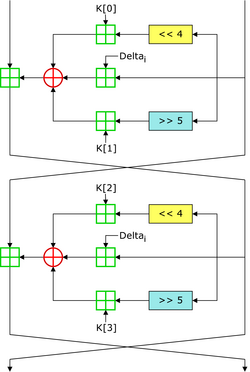
\includegraphics[width=6cm,height=\textheight]{images/crypto/TEA_InfoBox_Diagram.png}
\end{center}

\begin{tcolorbox}[enhanced jigsaw, toprule=.15mm, opacityback=0, colbacktitle=quarto-callout-important-color!10!white, breakable, colframe=quarto-callout-important-color-frame, title=\textcolor{quarto-callout-important-color}{\faExclamation}\hspace{0.5em}{(Fast) kein Feistel Netzwerk}, left=2mm, arc=.35mm, toptitle=1mm, bottomrule=.15mm, rightrule=.15mm, titlerule=0mm, bottomtitle=1mm, leftrule=.75mm, opacitybacktitle=0.6, coltitle=black, colback=white]

Die verschlüsselten Blöcke können nicht so einfach wieder entschlüsselt,
da im Algorithmus nebst XOR noch Additionen stattfinden. Für die
Entschlüsselung werden die \textbf{Addition rückgängig} mit
Subtraktionen gemacht.

\end{tcolorbox}

\subsection{XTEA}\label{xtea}

e\textbf{X}tended \textbf{TEA} ist eine Erweiterung von TEA, welcher die
Verschlüsselung besser macht. Gleiche Eigenschaften + Konstantwert
\texttt{delta=0x9E3779B9}.

\begin{center}
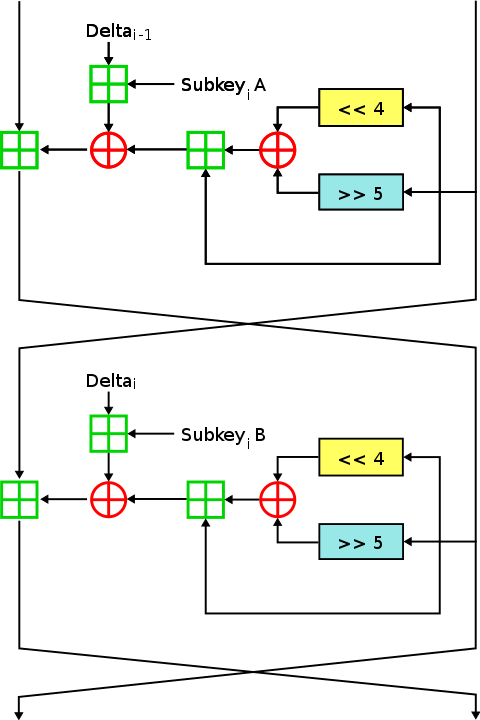
\includegraphics[width=6cm,height=\textheight]{images/crypto/XTEA_InfoBox_Diagram.png}
\end{center}

\begin{tcolorbox}[enhanced jigsaw, toprule=.15mm, opacityback=0, colbacktitle=quarto-callout-important-color!10!white, breakable, colframe=quarto-callout-important-color-frame, title=\textcolor{quarto-callout-important-color}{\faExclamation}\hspace{0.5em}{XTEA sicher?}, left=2mm, arc=.35mm, toptitle=1mm, bottomrule=.15mm, rightrule=.15mm, titlerule=0mm, bottomtitle=1mm, leftrule=.75mm, opacitybacktitle=0.6, coltitle=black, colback=white]

XTEA ist ein sicherer Verschlüsselungsalgorithmus, wenn auch nicht so
sicher wie RSA oder andere.

\end{tcolorbox}

\subsection{AES}\label{aes}

\subsection{\texorpdfstring{Cipher Modi
\href{https://en.wikipedia.org/wiki/Block_cipher_mode_of_operation\#CTR}{\faWikipediaW}}{Cipher Modi }}\label{cipher-modi}

\subsubsection{Electronic Code Book
(ECB)}\label{electronic-code-book-ecb}

\subsubsection{Cyber Block Chaining
(CBC)}\label{cyber-block-chaining-cbc}

\subsubsection{Cipiher FeedBack (CFB)}\label{cipiher-feedback-cfb}

\subsubsection{Output FeedBack (OFB)}\label{output-feedback-ofb}

\subsubsection{CounTeR (CTR)}\label{counter-ctr}

\subsubsection{Galois Counter Mode (GCM)}\label{galois-counter-mode-gcm}

\subsection{Meet-In-The-Middle Attack}\label{meet-in-the-middle-attack}

\subsection{Double Encrpytion}\label{double-encrpytion}

\subsection{Triple Encrpytion}\label{triple-encrpytion}

\subsection{Key Whitening}\label{key-whitening}

\subsection{Hash Functions}\label{hash-functions}

\subsubsection{Block}\label{block}

\subsection{weitere Begriffe}\label{weitere-begriffe}

{\small
\textbf{Keyspace} Anzahl möglichen \& relevanten Keys

\textbf{Brute Force} Alle Keykombination versuchen (Erfolg $\approx$ Keyspace/2)

\textbf{Frequency Analysis} Gewisse Zeichen(kombinationen) werden häufiger verwendet 

}

\newpage

\section{\texorpdfstring{Docker \faIcon{docker}}{Docker }}\label{docker}

\begin{center}

\includegraphics[width=7cm,height=\textheight]{images/meme_docker.jpg}
\end{center}

\begin{tcolorbox}[enhanced jigsaw, toprule=.15mm, opacityback=0, colbacktitle=quarto-callout-important-color!10!white, breakable, colframe=quarto-callout-important-color-frame, title=\textcolor{quarto-callout-important-color}{\faExclamation}\hspace{0.5em}{Wichtig}, left=2mm, arc=.35mm, toptitle=1mm, bottomrule=.15mm, rightrule=.15mm, titlerule=0mm, bottomtitle=1mm, leftrule=.75mm, opacitybacktitle=0.6, coltitle=black, colback=white]

Bash Befehle via Host sind mit {\color{BrickRed}{\texttt{\textbf{\$}}}}
gekennzeichnet.

\begin{Shaded}
\begin{Highlighting}[]
\ExtensionTok{\$}\NormalTok{ echo }\StringTok{"this happens on the host"}
\end{Highlighting}
\end{Shaded}

Bash Befehle in einem Docker Container sind mit
{\color{BrickRed}{\texttt{\textbf{\#}}}} gekennzeichnet.

\begin{Shaded}
\begin{Highlighting}[]
\ExtensionTok{\#}\NormalTok{ echo }\StringTok{"this happens in a Docker container"}
\end{Highlighting}
\end{Shaded}

\end{tcolorbox}

\subsection{Was'n Docka?}\label{wasn-docka}

Docker ist eine Plattform zur Software-Virtualisierung mit Fokus auf
\ul{Wiederverwendbarkeit} und \ul{Containerisierung}.

Die Idee ist, eine Anwendunge mit der nötigen Konfiguration, Runtime und
Bibliotheken in ein Paket zusammenzustellen und dann als
\textbf{portables} Produkt weitergegeben, verarbeitet, etc. ausgeführt
werden.

\subsection{Begriffe}\label{begriffe}

\begin{description}
\tightlist
\item[Image]
eine schreibgeschützte und vorgefertigte Vorlage, welche alle nötigen
Software and Dateien beinhaltet. Es ist eine ``Momentaufnahme'' des
Filesystems.
\item[Container]
ist die \ul{ausgeführte Instanz eines Images} und ist eine
\ul{isolierte} Umgebung, welche die entsprechende Prozesse ausführt,
\textbf{ohne} andere Systeme zu stören.
\item[Dockerfile]
beschreibt wie ein Docker Image zusammengebaut wird anhand Schritten
\(\rightarrow\) welche Tools installiert und Dateien kopiert werden
\item[Layers]
Ein Image ist auf Layern aufgebaut, welche während einem Build-Prozess
mit einem Dockerfile erstellt werden. Jede Anweisung im Dockerfile
erzeugt einen neuen Layer mit einer eindeutigen ID.
\item[Container Layer]
Wenn ein Container kreiert und gestartet wird, entsteht ein Container
Layer, welcher alle Änderungen verfolgt. Mit \texttt{commit} kann ein
neues Image mit diesen Änderungen kreiert werden.
\item[Docker daemon \texttt{dockerd} (Service)]
Auch bekannt als \emph{Docker Engine}. Zuständig für Ausführungen der
Container und Docker Kommandos.
\item[Volumes]
Dateien in Volumes bleiben nach Beendigung/Löschung des Containers
erhalten (für Datenaustausch z.B. zwischen Host \& Cont. oder
seriell/parralel Cont. zu Cont.)
\end{description}

\subsection{Docker Pfade}\label{docker-pfade}

\begin{itemize}
\tightlist
\item
  \texttt{/var/lib/docker/}: Hauptverzeichnis von Docker
\item
  \texttt{/var/lib/docker/images/}: enthält Metadaten zu den Images
\item
  \texttt{/var/lib/docker/\textless{}overlay-driver\textgreater{}/}:
  enthält ausgepackte Layer (Images \& Container)
\item
  \texttt{/var/lib/docker/volumes/}: enthält Volumen
\end{itemize}

\subsection{Images}\label{images}

Images sind \textbf{schreibgeschützte} Pakete, welches schichtenweise
mit Software und Strukturen aufgebaut ist.

\begin{center}
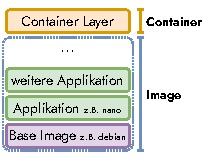
\includegraphics[width=6cm,height=\textheight]{images/docker/image_structure.pdf}
\end{center}

\subsubsection{\texorpdfstring{{\small \faTerminal\hspace{1mm}}
Auflisten}{ Auflisten}}\label{auflisten}

Listet alle heruntergeladenen Images auf

\begin{Shaded}
\begin{Highlighting}[]
\ExtensionTok{$}\NormalTok{ docker images}
\ExtensionTok{$}\NormalTok{ docker image ls}
\ExtensionTok{$}\NormalTok{ docker image list}
\ExtensionTok{REPOSITORY}\NormalTok{   TAG       IMAGE ID       CREATED       SIZE}
\ExtensionTok{debian}\NormalTok{       latest    5027089adc4c   3 weeks ago   117MB}
\end{Highlighting}
\end{Shaded}

\subsubsection{\texorpdfstring{{\small \faTerminal\hspace{1mm}}
Löschen}{ Löschen}}\label{luxf6schen}

\begin{Shaded}
\begin{Highlighting}[]
\ExtensionTok{$}\NormalTok{ docker rm }\OperatorTok{\textless{}}\NormalTok{image}\OperatorTok{\textgreater{}}
\ExtensionTok{$}\NormalTok{ docker images rm }\OperatorTok{\textless{}}\NormalTok{Image}\OperatorTok{\textgreater{}}
\ExtensionTok{$}\NormalTok{ docker rmi }\OperatorTok{\textless{}}\NormalTok{image}\OperatorTok{\textgreater{}}
\end{Highlighting}
\end{Shaded}

Löscht ein Image (\textcolor{RedOrange}{\textbf{WICHTIG}} kein Container
mit diesem Image sollte dabei existieren, sonst gehts nicht)

\begin{Shaded}
\begin{Highlighting}[]
\ExtensionTok{$}\NormalTok{ docker image prune}
\end{Highlighting}
\end{Shaded}

löscht \emph{dangling} (nicht gekennzeichnete / Tag = \texttt{none})
Images. \texttt{-a} löscht alle Images, welche nicht verwendet werden

\subsubsection{\texorpdfstring{{\small \faTerminal\hspace{1mm}} Neue
Version
veröffentlichen}{ Neue Version veröffentlichen}}\label{neue-version-veruxf6ffentlichen}

Nachdem eine Version kreiert wurde, kann diese auf DockerHub
veröffentlicht werden.

\begin{Shaded}
\begin{Highlighting}[]
\ExtensionTok{$}\NormalTok{ docker image push }\PreprocessorTok{[}\SpecialStringTok{options}\PreprocessorTok{]} \OperatorTok{\textless{}}\NormalTok{name}\OperatorTok{\textgreater{}}\PreprocessorTok{[}\SpecialStringTok{:tag}\PreprocessorTok{]}
\end{Highlighting}
\end{Shaded}

\subsubsection{\texorpdfstring{{\small \faTerminal\hspace{1mm}}
Grösse}{ Grösse}}\label{gruxf6sse}

{\small

\begin{Shaded}
\begin{Highlighting}[]
\ExtensionTok{$}\NormalTok{ docker images}
\ExtensionTok{REPOSITORY}\NormalTok{   TAG     IMAGE ID      CREATED        SIZE}
\ExtensionTok{alpine}\NormalTok{       latest  1d34ffeaf190  2 weeks ago    7.79MB}
\ExtensionTok{hello{-}world}\NormalTok{  latest  d2c94e258dcb  13 months ago  13.3kB}
\end{Highlighting}
\end{Shaded}

}

\subsubsection{\texorpdfstring{{\small \faTerminal\hspace{1mm}}
Informationen
abrufen}{ Informationen abrufen}}\label{informationen-abrufen}

\begin{Shaded}
\begin{Highlighting}[]
\ExtensionTok{$}\NormalTok{ docker inspect }\OperatorTok{\textless{}}\NormalTok{image}\OperatorTok{\textgreater{}}
\end{Highlighting}
\end{Shaded}

\subsection{Container}\label{container}

Container sind ausgeführte, \textbf{isolierte} Images.

\subsubsection{Container-Layer}\label{container-layer}

Da das Image schreibgeschützt ist, werden alle Änderungen, Löschungen
und Hinzufügungen am Image in der \textbf{Container-Layer} verfolgt
\(\rightarrow\) das Image bleibt heil und unversehen.

Dies bedeutet auch, dass das Image nur \textbf{einmal} pro Version
existiert.

\begin{center}
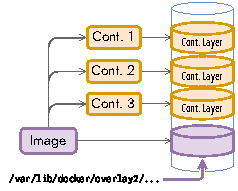
\includegraphics[width=7cm,height=\textheight]{images/docker/volume_clayer.pdf}
\end{center}

\subsubsection{\texorpdfstring{{\small \faTerminal\hspace{1mm}}
Erstellen/Ausführen/Starten}{ Erstellen/Ausführen/Starten}}\label{erstellenausfuxfchrenstarten}

\phantomsection\label{annotated-cell-7}%
\begin{Shaded}
\begin{Highlighting}[]
\ExtensionTok{$}\NormalTok{ docker run }\OperatorTok{\textless{}}\NormalTok{opt}\OperatorTok{\textgreater{}} \OperatorTok{\textless{}}\NormalTok{image}\OperatorTok{\textgreater{}} \OperatorTok{\textless{}}\NormalTok{args}\OperatorTok{\textgreater{}} \hspace*{\fill}\NormalTok{\circled{1}}
\ExtensionTok{$}\NormalTok{ docker create }\OperatorTok{\textless{}}\NormalTok{opt}\OperatorTok{\textgreater{}} \OperatorTok{\textless{}}\NormalTok{image}\OperatorTok{\textgreater{}} \OperatorTok{\textless{}}\NormalTok{args}\OperatorTok{\textgreater{}} \hspace*{\fill}\NormalTok{\circled{2}}
\ExtensionTok{$}\NormalTok{ docker start }\OperatorTok{\textless{}}\NormalTok{container}\OperatorTok{\textgreater{}}
\end{Highlighting}
\end{Shaded}

\begin{description}
\tightlist
\item[\circled{1}]
Direkt erstellen \& ausführen
\item[\circled{2}]
Container erstellen und dann ausführen
\end{description}

\subsubsection{\texorpdfstring{{\small \faTerminal\hspace{1mm}}
Auflisten}{ Auflisten}}\label{auflisten-1}

listet alle \textbf{momentan} ausgeführten Container auf. Mit
\texttt{-a} listet alle Container auf

\begin{Shaded}
\begin{Highlighting}[]
\ExtensionTok{$}\NormalTok{ docker ps }\CommentTok{\# kurz für \textquotesingle{}docker container ls\textquotesingle{}}
\ExtensionTok{CONTAINER}\NormalTok{ ID  IMAGE   COMMAND ... STATUS        ... NAMES}
\ExtensionTok{79f3f8a71b46}\NormalTok{  debian  }\StringTok{"bash"}\NormalTok{  ... Up 56 minutes ... musing\_wozniak}
\ExtensionTok{6201bc70ef8c}\NormalTok{  debian  }\StringTok{"bash"}\NormalTok{  ... Up 58 minutes ... magical\_villani}
\end{Highlighting}
\end{Shaded}

\subsubsection{\texorpdfstring{{\small \faTerminal\hspace{1mm}}
Attach/Detach}{ Attach/Detach}}\label{attachdetach}

Ein Container mit einer Shell, z.B. Bash, kann via \texttt{attach} oder
\texttt{-it} zugegriffen werden.

\phantomsection\label{annotated-cell-9}%
\begin{Shaded}
\begin{Highlighting}[]
\ExtensionTok{docker}\NormalTok{ attach }\OperatorTok{\textless{}}\NormalTok{container}\OperatorTok{\textgreater{}} \hspace*{\fill}\NormalTok{\circled{1}}
\ExtensionTok{docker}\NormalTok{ run }\AttributeTok{{-}it} \OperatorTok{\textless{}}\NormalTok{image}\OperatorTok{\textgreater{}} \hspace*{\fill}\NormalTok{\circled{2}}
\end{Highlighting}
\end{Shaded}

\begin{description}
\tightlist
\item[\circled{1}]
Bei bereits aktiven Container
\item[\circled{2}]
Die Shell des Containers wird an den Vordergrund gebracht + Pseudo
Terminal
\end{description}

Mit \texttt{CTRL+Q\ CTRL+P} hängt man sich vom Container ab, ohne ihn zu
beenden. \texttt{CTRL+C} oder im Shell \texttt{exit} beendet den
Container.

\subsubsection{\texorpdfstring{{\small \faTerminal\hspace{1mm}}
Interaktivität}{ Interaktivität}}\label{interaktivituxe4t}

Ein Container kann auf verschiedene Arten gestartet werden.

\phantomsection\label{annotated-cell-10}%
\begin{Shaded}
\begin{Highlighting}[]
\ExtensionTok{$}\NormalTok{ docker start }\OperatorTok{\textless{}}\NormalTok{container}\OperatorTok{\textgreater{}} \hspace*{\fill}\NormalTok{\circled{1}}
\ExtensionTok{$}\NormalTok{ docker start }\AttributeTok{{-}i} \OperatorTok{\textless{}}\NormalTok{container}\OperatorTok{\textgreater{}} \hspace*{\fill}\NormalTok{\circled{2}}
\end{Highlighting}
\end{Shaded}

\begin{description}
\tightlist
\item[\circled{1}]
im Hintergrund
\item[\circled{2}]
im Vordergrund
\end{description}

{\small

\begin{description}
\tightlist
\item[\texttt{-i/-\/-interactive}]
Macht den Container interaktiv und verbindet die Standardeingabe.
\item[\texttt{-t/-\/-tty}]
Aktiviert einen Pseudo-Terminalsimulator für den Container
(\texttt{...:/\#\ \textless{}cmd\textgreater{}}).
\end{description}

}

\phantomsection\label{annotated-cell-11}%
\begin{Shaded}
\begin{Highlighting}[]
\ExtensionTok{$}\NormalTok{ docker run }\AttributeTok{{-}i}\NormalTok{ debian }\hspace*{\fill}\NormalTok{\circled{1}}
\BuiltInTok{echo}\NormalTok{ hello world}
\ExtensionTok{hello}\NormalTok{ world}

\ExtensionTok{$}\NormalTok{ docker run }\AttributeTok{{-}it}\NormalTok{ debian }\hspace*{\fill}\NormalTok{\circled{2}}
\ExtensionTok{root@containerID:/\#}\NormalTok{ echo hello world}
\ExtensionTok{hello}\NormalTok{ world}

\ExtensionTok{$}\NormalTok{ docker create }\AttributeTok{{-}t}\NormalTok{ debian }\hspace*{\fill}\NormalTok{\circled{3}}
\ExtensionTok{$}\NormalTok{ docker start }\AttributeTok{{-}i} \OperatorTok{\textless{}}\NormalTok{container}\OperatorTok{\textgreater{}}
\end{Highlighting}
\end{Shaded}

\begin{description}
\tightlist
\item[\circled{1}]
Interaktiv ohne TTY
\item[\circled{2}]
Interaktiv mit TTY
\item[\circled{3}]
In Einzelschritten
\end{description}

\subsubsection{\texorpdfstring{{\small \faTerminal\hspace{1mm}}
Löschen}{ Löschen}}\label{luxf6schen-1}

\begin{Shaded}
\begin{Highlighting}[]
\ExtensionTok{$}\NormalTok{ docker rm }\OperatorTok{\textless{}}\NormalTok{container}\OperatorTok{\textgreater{}}\NormalTok{ [container ...]}
\end{Highlighting}
\end{Shaded}

Es können nur \emph{stopped} und \emph{created} Container gelöscht
werden.

\begin{tcolorbox}[enhanced jigsaw, toprule=.15mm, opacityback=0, colbacktitle=quarto-callout-tip-color!10!white, breakable, colframe=quarto-callout-tip-color-frame, title=\textcolor{quarto-callout-tip-color}{\faLightbulb}\hspace{0.5em}{Löschen nach Beendung}, left=2mm, arc=.35mm, toptitle=1mm, bottomrule=.15mm, rightrule=.15mm, titlerule=0mm, bottomtitle=1mm, leftrule=.75mm, opacitybacktitle=0.6, coltitle=black, colback=white]

\begin{Shaded}
\begin{Highlighting}[]
\ExtensionTok{$}\NormalTok{ docker run }\AttributeTok{{-}{-}rm} \OperatorTok{\textless{}}\NormalTok{image}\OperatorTok{\textgreater{}}
\end{Highlighting}
\end{Shaded}

\end{tcolorbox}

\begin{tcolorbox}[enhanced jigsaw, toprule=.15mm, opacityback=0, colbacktitle=quarto-callout-tip-color!10!white, breakable, colframe=quarto-callout-tip-color-frame, title=\textcolor{quarto-callout-tip-color}{\faLightbulb}\hspace{0.5em}{Inaktive Container löschen}, left=2mm, arc=.35mm, toptitle=1mm, bottomrule=.15mm, rightrule=.15mm, titlerule=0mm, bottomtitle=1mm, leftrule=.75mm, opacitybacktitle=0.6, coltitle=black, colback=white]

Löscht alle Container, welche nicht mehr verwendet werden.

\begin{Shaded}
\begin{Highlighting}[]
\ExtensionTok{$}\NormalTok{ docker container prune}
\end{Highlighting}
\end{Shaded}

\end{tcolorbox}

\subsubsection{\texorpdfstring{{\small \faTerminal\hspace{1mm}}
(Um-)benennen}{ (Um-)benennen}}\label{um-benennen}

Ein Name kann auf zwei Arten einem Container zugewiesen werden.

\phantomsection\label{annotated-cell-13}%
\begin{Shaded}
\begin{Highlighting}[]
\ExtensionTok{$}\NormalTok{ docker rename }\OperatorTok{\textless{}}\NormalTok{old}\OperatorTok{\textgreater{}} \OperatorTok{\textless{}}\NormalTok{new}\OperatorTok{\textgreater{}} \hspace*{\fill}\NormalTok{\circled{1}}
\ExtensionTok{$}\NormalTok{ docker run }\AttributeTok{{-}{-}name}\NormalTok{ peter\_enis debian }\hspace*{\fill}\NormalTok{\circled{2}}
\end{Highlighting}
\end{Shaded}

\begin{description}
\tightlist
\item[\circled{1}]
Ein bereits existierender Container wird umbenannt
\item[\circled{2}]
Bei \textbf{Erstellung} eines Containers kann direkt ein Name zugewiesen
werden
\end{description}

\subsubsection{\texorpdfstring{{\small \faTerminal\hspace{1mm}} Dateien
kopieren Host \(\rightleftarrows\)
Container}{ Dateien kopieren Host \textbackslash rightleftarrows Container}}\label{dateien-kopieren-host-rightleftarrows-container}

Der Docker Host kann Dateien in und aus dem Container kopieren.

\phantomsection\label{annotated-cell-14}%
\begin{Shaded}
\begin{Highlighting}[]
\ExtensionTok{$}\NormalTok{ docker container cp }\OperatorTok{\textless{}}\NormalTok{container}\OperatorTok{\textgreater{}}\NormalTok{:}\OperatorTok{\textless{}}\NormalTok{path}\OperatorTok{\textgreater{}} \OperatorTok{\textless{}}\NormalTok{dest}\OperatorTok{\textgreater{}} \hspace*{\fill}\NormalTok{\circled{1}}
\ExtensionTok{$}\NormalTok{ docker cp }\OperatorTok{\textless{}}\NormalTok{src}\OperatorTok{\textgreater{}} \OperatorTok{\textless{}}\NormalTok{container}\OperatorTok{\textgreater{}}\NormalTok{:}\OperatorTok{\textless{}}\NormalTok{dest}\OperatorTok{\textgreater{}} \hspace*{\fill}\NormalTok{\circled{2}}
\end{Highlighting}
\end{Shaded}

\begin{description}
\tightlist
\item[\circled{1}]
kopiert dateien vom Container zum Host
\item[\circled{2}]
kopiert vom Host zum Container
\end{description}

\subsubsection{\texorpdfstring{{\small \faTerminal\hspace{1mm}}
Ausgabe}{ Ausgabe}}\label{ausgabe}

Zeigt Log Daten (z.B. Konsolenausgabe) während der Ausführung an
(\texttt{-f} folgt dem Container/ kontinuierliches Update)

\begin{Shaded}
\begin{Highlighting}[]
\ExtensionTok{$}\NormalTok{ docker logs }\OperatorTok{\textless{}}\NormalTok{container}\OperatorTok{\textgreater{}}
\end{Highlighting}
\end{Shaded}

\subsubsection{\texorpdfstring{{\small \faTerminal\hspace{1mm}} Prozesse
ausführen/abfragen}{ Prozesse ausführen/abfragen}}\label{prozesse-ausfuxfchrenabfragen}

Führt Prozesse in einem aktiven Container aus.

\begin{Shaded}
\begin{Highlighting}[]
\ExtensionTok{$}\NormalTok{ docker exec }\OperatorTok{\textless{}}\NormalTok{container}\OperatorTok{\textgreater{}} \OperatorTok{\textless{}}\NormalTok{cmd}\OperatorTok{\textgreater{}}
\end{Highlighting}
\end{Shaded}

Gibt Prozesse des Containers an (\texttt{ax} als Argument gibt alle
laufenden Prozesse an)

\begin{Shaded}
\begin{Highlighting}[]
\ExtensionTok{$}\NormalTok{ docker top }\OperatorTok{\textless{}}\NormalTok{container}\OperatorTok{\textgreater{}} \OperatorTok{\textless{}}\NormalTok{arg}\OperatorTok{\textgreater{}}
\ExtensionTok{$}\NormalTok{ docker container top }\OperatorTok{\textless{}}\NormalTok{container}\OperatorTok{\textgreater{}} \OperatorTok{\textless{}}\NormalTok{arg}\OperatorTok{\textgreater{}}
\end{Highlighting}
\end{Shaded}

\subsubsection{\texorpdfstring{{\small \faTerminal\hspace{1mm}}
Logging}{ Logging}}\label{logging}

Zeigt Log Daten während ausführung an (\texttt{-f} folgt dem Container/
kontinuierliches update).

\begin{Shaded}
\begin{Highlighting}[]
\ExtensionTok{$}\NormalTok{ docker logs }\OperatorTok{\textless{}}\NormalTok{container}\OperatorTok{\textgreater{}}
\end{Highlighting}
\end{Shaded}

\subsubsection{Lebenszyklus}\label{lebenszyklus}

Ein Docker-\textbf{Container} kann fünf Zustände annehmen (\ul{Created},
\ul{Running}, \ul{Deleted}, \ul{Stopped} und \ul{Paused}) und kann mit
folgenden Docker-Befehlen gesteuert werden.

\resizebox{\columnwidth}{!}{
  \begin{tikzpicture}[line/.style={-Straight Barb,shorten >=1mm,shorten <=1mm,draw=black}, label/.style={fill=white},  node font=\ttfamily]

\node[circle,draw=black, inner sep=0, minimum width=1.4cm] (stateRunning) at (4,6) {running};
\node[circle,draw=black, inner sep=0, minimum width=1.4cm] (stateStopped) at (4,2) {stopped};
\node[circle,draw=black, inner sep=0, minimum width=1.4cm] (stateDeleted) at (0,2) {deleted};
\node[circle,draw=black, inner sep=0, minimum width=1.4cm] (stateCreated) at (0,6) {created};
\node[circle,draw=black, inner sep=0, minimum width=1.4cm] (statePaused)  at (8,6) {paused};

\node (entry1) at (-3,6) {};
\node (entry2) at (4,8) {};

\draw [line, rounded corners=5,gray] (stateRunning) .. controls (3.25,4.75) and (3.25,2.75) .. ([yshift=5mm]stateStopped.center) .. controls (4.75,2.75) and (4.75,4.75) .. (stateRunning);


\draw [line]                (stateCreated) edge node[label]        {start}  (stateRunning);
\draw [line,bend right=5mm] (stateRunning) edge node[label,left=1pt]  {stop}   (stateStopped);
\draw [line,bend right=5mm] (stateStopped) edge node[label,right=1pt] {start}  (stateRunning);

\draw [line,bend right=5mm] (stateRunning) edge node[label]       {pause}   (statePaused);
\draw [line,bend right=5mm] (statePaused)  edge node[label]       {unpause} (stateRunning);
\draw [line]                (stateCreated) edge node[label]       {rm}      (stateDeleted);
\draw [line]                (stateStopped) edge node[label]       {rm}      (stateDeleted);

\draw [line]                (entry1)       edge node[label]       {create}  (stateCreated);
\draw [line]                (entry2)       edge node[label]       {run}     (stateRunning);
\node [label,left, fill=none] at (3.25,4.75) {restart};
\end{tikzpicture}
}

\begin{tcolorbox}[enhanced jigsaw, toprule=.15mm, opacityback=0, colbacktitle=quarto-callout-note-color!10!white, breakable, colframe=quarto-callout-note-color-frame, title=\textcolor{quarto-callout-note-color}{\faInfo}\hspace{0.5em}{Unterschied \emph{Stopped} und \emph{Paused}}, left=2mm, arc=.35mm, toptitle=1mm, bottomrule=.15mm, rightrule=.15mm, titlerule=0mm, bottomtitle=1mm, leftrule=.75mm, opacitybacktitle=0.6, coltitle=black, colback=white]

Wenn ein Container gestoppt wird, werden alle ihm zugewiesenen
Ressourcen freigegeben, während bei einem angehaltenen Container kein
Speicher, aber die CPU freigegeben wird.

\end{tcolorbox}

\subsubsection{\texorpdfstring{{\small \faTerminal\hspace{1mm}} Grösse
\texttt{-\/-size}}{ Grösse -\/-size}}\label{gruxf6sse---size}

Da ein Container Änderungen auf einer separaten Layer verfolgt, ist der
Speicherplatz selbst meistens klein.

{\small

\begin{Shaded}
\begin{Highlighting}[]
\ExtensionTok{$}\NormalTok{ docker ps }\AttributeTok{{-}a} \AttributeTok{{-}{-}size}
\ExtensionTok{CONTAINER}\NormalTok{ ID   IMAGE       ...  NAMES               SIZE}
\ExtensionTok{253be0a7fe55}\NormalTok{   alpine      ...  brave\_pascal        8B }\ErrorTok{(}\ExtensionTok{virtual}\NormalTok{ 7.79MB}\KeywordTok{)}
\ExtensionTok{68bb3a7fdf37}\NormalTok{   hello{-}world ...  loving\_mcclintock   0B }\ErrorTok{(}\ExtensionTok{virtual}\NormalTok{ 13.3kB}\KeywordTok{)}
\ExtensionTok{d20695e9fe4b}\NormalTok{   alpine      ...  unruffled\_tesla     25B }\ErrorTok{(}\ExtensionTok{virtual}\NormalTok{ 7.79MB}\KeywordTok{)}
\end{Highlighting}
\end{Shaded}

}

\texttt{virtual} referenziert auf Container + Image = Totale
theoretische Grösse.

\subsubsection{Image kreieren aus
Container}\label{image-kreieren-aus-container}

Aus einem Container kann ein neues Image erstellt werden:

\begin{Shaded}
\begin{Highlighting}[]
\ExtensionTok{$}\NormalTok{ docker container commit }\OperatorTok{\textless{}}\NormalTok{container}\OperatorTok{\textgreater{}}\NormalTok{ [image}\PreprocessorTok{[}\SpecialStringTok{:tag}\PreprocessorTok{]}\NormalTok{]}
\ExtensionTok{$}\NormalTok{ docker commit ...}
\end{Highlighting}
\end{Shaded}

\subsection{Volume}\label{volume}

Container sind voneinander isoliert \(\rightarrow\) Datenaustausch
zwischen Host \(\rightleftarrows\) Container \& Container
\(\rightleftarrows\) Container wird mit \textbf{Volumen} gemacht. Dies
muss \textbf{explizit} angegeben werden.

\begin{center}
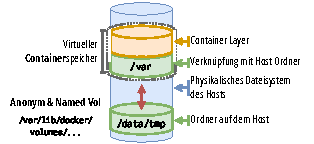
\includegraphics[width=9cm,height=\textheight]{images/docker/volume_structure.pdf}
\end{center}

Mit dem Parameter \AttributeTok{{-}v} und einem Pfad wird ein Volumen
angegeben.

\subsubsection{Host Volumes}\label{host-volumes}

\begin{Shaded}
\begin{Highlighting}[]
\ExtensionTok{$}\NormalTok{ docker run }\AttributeTok{{-}v}\NormalTok{ /path/in/host:/path/in/container }\OperatorTok{\textless{}}\NormalTok{opt}\OperatorTok{\textgreater{}} \OperatorTok{\textless{}}\NormalTok{image}\OperatorTok{\textgreater{}}
\end{Highlighting}
\end{Shaded}

\begin{itemize}
\tightlist
\item
  \texttt{/path/in/host}: Pfad auf dem Host
\item
  \texttt{/path/in/container}: Pfad im Container, welche mit dem
  Host-Pfad verbunden wird.
\end{itemize}

\subsubsection{Named Volumes}\label{named-volumes}

\begin{Shaded}
\begin{Highlighting}[]
\ExtensionTok{$}\NormalTok{ docker run }\AttributeTok{{-}v}\NormalTok{ name:/path/in/container }\OperatorTok{\textless{}}\NormalTok{opt}\OperatorTok{\textgreater{}} \OperatorTok{\textless{}}\NormalTok{image}\OperatorTok{\textgreater{}}
\end{Highlighting}
\end{Shaded}

\begin{itemize}
\tightlist
\item
  \texttt{name}: Name des Volumens
\item
  \texttt{/path/in/container}: Pfad im Container, welche geöffnet wird.
\end{itemize}

\subsubsection{Anonyme Volumes}\label{anonyme-volumes}

\begin{Shaded}
\begin{Highlighting}[]
\ExtensionTok{$}\NormalTok{ docker run }\AttributeTok{{-}v}\NormalTok{ /path/in/container }\OperatorTok{\textless{}}\NormalTok{opt}\OperatorTok{\textgreater{}} \OperatorTok{\textless{}}\NormalTok{image}\OperatorTok{\textgreater{}}
\end{Highlighting}
\end{Shaded}

\begin{itemize}
\tightlist
\item
  \texttt{/path/in/container}: Pfad im Container, welche geöffnet wird.
\end{itemize}

\subsubsection{Datenaustasch}\label{datenaustasch}

\circled{1} \ul{Host \& Container}

\begin{center}
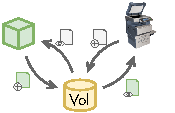
\includegraphics[width=6cm,height=\textheight]{images/docker/volume_exchange_host.pdf}
\end{center}

\circled{2} \ul{Container \& Container (parallel)}

\begin{center}
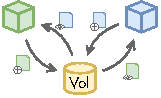
\includegraphics[width=6cm,height=\textheight]{images/docker/volume_exchange_parallel.pdf}
\end{center}

\circled{3} \ul{Container nach Container (seriell)}

\begin{center}
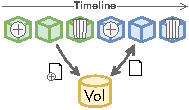
\includegraphics[width=6cm,height=\textheight]{images/docker/volume_exchange_series.pdf}
\end{center}

\subsubsection{Speicherpfade}\label{speicherpfade}

\ul{Benannte} \& \ul{anonyme} Volumen werden unter dem Pfad
\texttt{/var/lib/docker/volumes/} angelegt.

\ul{Host} Volumen werden an einem vom Host festgelegten Pfad angelegt.

\subsubsection{\texorpdfstring{{\small \faTerminal\hspace{1mm}}
Auflisten}{ Auflisten}}\label{auflisten-2}

\begin{Shaded}
\begin{Highlighting}[]
\ExtensionTok{$}\NormalTok{ docker volume ls}
\end{Highlighting}
\end{Shaded}

\subsubsection{\texorpdfstring{{\small \faTerminal\hspace{1mm}} Volumen
löschen}{ Volumen löschen}}\label{volumen-luxf6schen}

Um ein Volumen zu löschen, muss der Name des Volumens angegeben werden.
Ebenfalls darf es von keinem Container verwendet werden.

\begin{Shaded}
\begin{Highlighting}[]
\ExtensionTok{$}\NormalTok{ docker volume rm }\OperatorTok{\textless{}}\NormalTok{volume}\OperatorTok{\textgreater{}}
\end{Highlighting}
\end{Shaded}

\texttt{prune} löscht nicht gebrauchte \ul{anonyme} Volumen. Mit
\texttt{-a/-\/-all} können ungebrauchte \ul{anonyme und benannte}
Volumen gelöscht werden.

\begin{Shaded}
\begin{Highlighting}[]
\ExtensionTok{$}\NormalTok{ docker volume prune}
\end{Highlighting}
\end{Shaded}

\subsubsection{\texorpdfstring{{\small \faTerminal\hspace{1mm}}
Erstellen}{ Erstellen}}\label{erstellen}

Mit dem \texttt{volume\ create} Befehl können anonyme und benannte
Volumen erstellt werden. Einfach keine Pfad/Host Volumen.

\begin{Shaded}
\begin{Highlighting}[]
\ExtensionTok{$}\NormalTok{ docker volume create }\PreprocessorTok{[}\SpecialStringTok{name}\PreprocessorTok{]}
\end{Highlighting}
\end{Shaded}

\subsection{Dockerfile}\label{dockerfile}

Mit einem \faFile[regular] \texttt{Dockerfile} kann ein Image erstellt
werden anhand Anweisungen. \ul{Jede Anweisung erzeugt eine eigene
Layer}.

\begin{center}
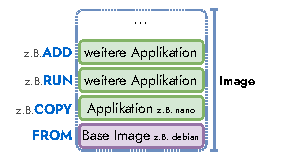
\includegraphics[width=8cm,height=\textheight]{images/docker/dockerfile_image.pdf}
\end{center}

\subsubsection{Anweisungen}\label{anweisungen}

\begin{Shaded}
\begin{Highlighting}[]
\KeywordTok{FROM}\NormalTok{ \textless{}image\textgreater{} }\CommentTok{\# image oder \textquotesingle{}scratch\textquotesingle{}}
\end{Highlighting}
\end{Shaded}

Mit der Anweisung \texttt{FROM} setzt man das Parent- oder Basis-Image.
Es ist die erste Anweisung in einem Dockerfiles. Es können mehrere
\texttt{FROM} verwendet werden, wenn man Multistage-Building machen
möchte.

\begin{Shaded}
\begin{Highlighting}[]
\KeywordTok{COPY}\NormalTok{ [OPTIONS] \textless{}src\textgreater{} ... \textless{}dest\textgreater{}}
\KeywordTok{COPY}\NormalTok{ [OPTIONS] [}\StringTok{"\textless{}src\textgreater{}"}\NormalTok{, ... }\StringTok{"\textless{}dest\textgreater{}"}\NormalTok{]}
\end{Highlighting}
\end{Shaded}

Kopiert die Quelle zur Destination. Wenn die Destination ein Ordner ist,
können mehrer Dateien kopiert werden. Mit dem Wildcard-Zeichen\texttt{*}
und Wildcard-Einzelzeichen \texttt{?} können mehrere ähnliche Dateien
auf einmal kopiert werden.

\begin{Shaded}
\begin{Highlighting}[]
\KeywordTok{COPY}\NormalTok{ hom*.txt /mydir/}
\CommentTok{\# sammelt alle Dateien z.B. \textquotesingle{}home.txt\textquotesingle{} und \textquotesingle{}homie.txt\textquotesingle{}}

\KeywordTok{COPY}\NormalTok{ hom?.txt /mydir/}
\CommentTok{\# findet \textquotesingle{}home.txt\textquotesingle{}, aber nicht \textquotesingle{}homie.txt\textquotesingle{}}
\end{Highlighting}
\end{Shaded}

\begin{Shaded}
\begin{Highlighting}[]
\KeywordTok{RUN}\NormalTok{ [OPTIONS] \textless{}command\textgreater{} ...}
\KeywordTok{RUN}\NormalTok{ [OPTIONS] [ }\StringTok{"\textless{}command\textgreater{}"}\NormalTok{, ... ]}
\end{Highlighting}
\end{Shaded}

Führt Befehle im Image aus, z.B.
\VERB|\KeywordTok{RUN} \ExtensionTok{apt{-}get}\NormalTok{ update }\KeywordTok{\&\&} \ExtensionTok{apt{-}get}\NormalTok{ install }\AttributeTok{{-}y}\NormalTok{ curl}|.
Mit \texttt{\textbackslash{}} kann der Befehl auf mehrere Zeilen
gebrochen werden.

\begin{Shaded}
\begin{Highlighting}[]
\KeywordTok{ADD}\NormalTok{ [OPTIONS] \textless{}src\textgreater{} ... \textless{}dest\textgreater{}}
\KeywordTok{ADD}\NormalTok{ [OPTIONS] [}\StringTok{"\textless{}src\textgreater{}"}\NormalTok{, ... }\StringTok{"\textless{}dest\textgreater{}"}\NormalTok{]}
\end{Highlighting}
\end{Shaded}

Ähnlich wie \texttt{COPY}, einfach können URLs angegeben werden und
gezippte Dateien werden automatisch entpackt.

\subsubsection{Startkommando}\label{startkommando}

Die Startkommandos eines Container können auf zwei Arten gesetzt:
\texttt{CMD} und \texttt{ENTRYPOINT}.

\begin{Shaded}
\begin{Highlighting}[]
\KeywordTok{ENTRYPOINT}\NormalTok{ [}\StringTok{"executable"}\NormalTok{, }\StringTok{"param1"}\NormalTok{, }\StringTok{"param2"}\NormalTok{]}
\KeywordTok{ENTRYPOINT} \BuiltInTok{command}\NormalTok{ param1 param2}
\end{Highlighting}
\end{Shaded}

\begin{Shaded}
\begin{Highlighting}[]
\CommentTok{\# wenn ENTRYPOINT nicht gesetzt ist, wird CMD als Startkommande verwendet.}
\KeywordTok{CMD}\NormalTok{ [}\StringTok{"executable"}\NormalTok{,}\StringTok{"param1"}\NormalTok{,}\StringTok{"param2"}\NormalTok{]}

\CommentTok{\# als default Parameter zu ENTRYPOINT}
\KeywordTok{CMD}\NormalTok{ [}\StringTok{"param1"}\NormalTok{,}\StringTok{"param2"}\NormalTok{]}
\end{Highlighting}
\end{Shaded}

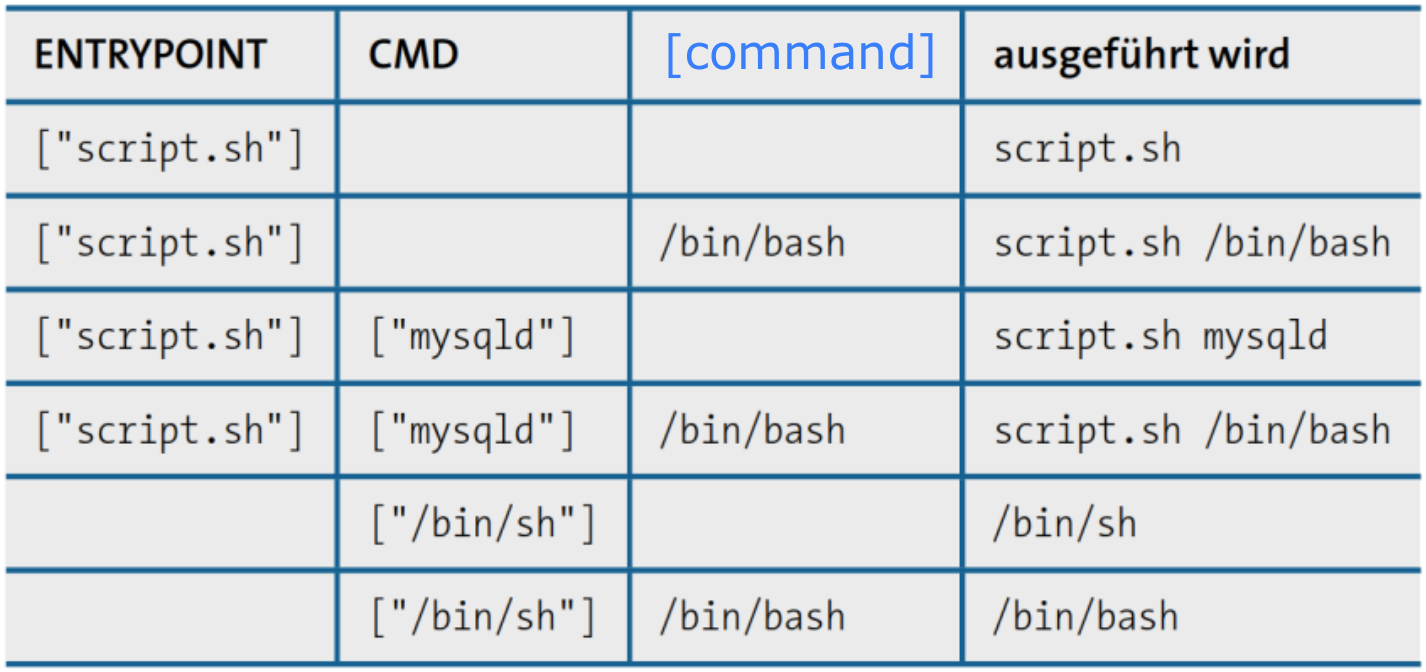
\includegraphics{images/docker/image-1.png}

\begin{Shaded}
\begin{Highlighting}[]
\ExtensionTok{$}\NormalTok{ docker run }\PreprocessorTok{[}\SpecialStringTok{opts}\PreprocessorTok{]} \OperatorTok{\textless{}}\NormalTok{image}\OperatorTok{\textgreater{}} \PreprocessorTok{[}\SpecialStringTok{command}\PreprocessorTok{]} \PreprocessorTok{[}\SpecialStringTok{args...}\PreprocessorTok{]}
\ExtensionTok{$}\NormalTok{ docker run }\AttributeTok{{-}{-}rm} \AttributeTok{{-}it}\NormalTok{ debian ls }\AttributeTok{{-}la} \CommentTok{\# startet "ls {-}la" im Container}
\end{Highlighting}
\end{Shaded}

Um die Startkommandos eines Images anzuzeigen

\begin{Shaded}
\begin{Highlighting}[]
\ExtensionTok{$}\NormalTok{ docker inspect }\AttributeTok{{-}f} \StringTok{\textquotesingle{}ENTRYPOINT:\{\{.Config.Entrypoint\}\}; CMD:\{\{.Config.Cmd\}\}\textquotesingle{}} \OperatorTok{\textless{}}\NormalTok{image}\OperatorTok{\textgreater{}}
\StringTok{"ENTRYPOINT:[]; CMD:[bash]"}

\ExtensionTok{$}\NormalTok{ docker inspect }\AttributeTok{{-}f} \StringTok{\textquotesingle{}ENTRYPOINT:\{\{.Config.Entrypoint\}\}; CMD:\{\{.Config.Cmd\}\}\textquotesingle{}}\NormalTok{ kaohslu/01{-}demo{-}img}
\StringTok{"ENTRYPOINT:[dotnet ASYD\_Demo.dll]; CMD:[]"}
\end{Highlighting}
\end{Shaded}

\begin{Shaded}
\begin{Highlighting}[]
\KeywordTok{WORKDIR}\NormalTok{ /path/to/workdir}
\end{Highlighting}
\end{Shaded}

Mit \texttt{WORKDIR} wird der Arbeitspfad gesetzt (ab Aufruf der
Anweisung), wo Befehle wie \texttt{COPY} oder \texttt{ADD} ihre Arbeit
verrichten.

\subsubsection{Image builden}\label{image-builden}

\begin{Shaded}
\begin{Highlighting}[]
\ExtensionTok{$}\NormalTok{ docker build }\OperatorTok{\textless{}}\NormalTok{path}\OperatorTok{\textgreater{}}\NormalTok{ {-}t }\OperatorTok{\textless{}}\NormalTok{name}\OperatorTok{\textgreater{}}\NormalTok{:}\OperatorTok{\textless{}}\NormalTok{tag}\OperatorTok{\textgreater{}}
\ExtensionTok{$}\NormalTok{ docker build }\AttributeTok{{-}t} \OperatorTok{\textless{}}\NormalTok{name}\OperatorTok{\textgreater{}}\NormalTok{:}\OperatorTok{\textless{}}\NormalTok{tag}\OperatorTok{\textgreater{}} \OperatorTok{\textless{}}\NormalTok{path}\OperatorTok{\textgreater{}}
\end{Highlighting}
\end{Shaded}

\subsubsection{Image Build History
zeigen}\label{image-build-history-zeigen}

Um die History eines Images anzuschauen \(\rightarrow\) Wie das Image
erstellt wurde.

\begin{Shaded}
\begin{Highlighting}[]
\ExtensionTok{$}\NormalTok{ docker history }\OperatorTok{\textless{}}\NormalTok{image}\OperatorTok{\textgreater{}}
\end{Highlighting}
\end{Shaded}

\subsubsection{Multistage}\label{multistage}

Mit Multistage Building können komplexe Images erzeugt werden.

\begin{Shaded}
\begin{Highlighting}[]
\CommentTok{\# }\CommentVarTok{syntax=docker/dockerfile:1}
\KeywordTok{FROM}\NormalTok{ golang:1.21}
\CommentTok{\# FROM golang:1.21 as build}
\KeywordTok{WORKDIR}\NormalTok{ /src}
\KeywordTok{COPY}\NormalTok{ \textless{}\textless{}EOF ./main.go}
\NormalTok{package main}

\NormalTok{import }\StringTok{"fmt"}

\NormalTok{func main() \{}
\NormalTok{  fmt.Println(}\StringTok{"hello, world"}\NormalTok{)}
\NormalTok{\}}
\NormalTok{EOF}
\KeywordTok{RUN} \ExtensionTok{go}\NormalTok{ build }\AttributeTok{{-}o}\NormalTok{ /bin/hello ./main.go}

\KeywordTok{FROM}\NormalTok{ scratch}
\KeywordTok{COPY} \OperatorTok{{-}{-}from=0}\NormalTok{ /bin/hello /bin/hello}
\CommentTok{\# COPY {-}{-}from=build /bin/hello /bin/hello}
\KeywordTok{CMD}\NormalTok{ [}\StringTok{"/bin/hello"}\NormalTok{]}
\end{Highlighting}
\end{Shaded}

\subsection{Netzwerke}\label{netzwerke}

Da Container per default isoliert sind (laufen in einem privaten
Netzwerk, welches sich Docker kümmert), muss man z.B. Netzwerke
\textbf{explizit} nach aussen öffnen, wenn man das will.

\textcolor{BrickRed}{[\textbf{TODO?}]}

\subsection{Docker Hub}\label{docker-hub}

\subsubsection{Images suchen \&
herunterladen}\label{images-suchen-herunterladen}

\begin{Shaded}
\begin{Highlighting}[]
\ExtensionTok{$}\NormalTok{ docker search }\OperatorTok{\textless{}}\NormalTok{searchterm}\OperatorTok{\textgreater{}}
\end{Highlighting}
\end{Shaded}

\begin{Shaded}
\begin{Highlighting}[]
\ExtensionTok{$}\NormalTok{ docker pull }\OperatorTok{\textless{}}\NormalTok{image}\OperatorTok{\textgreater{}}
\end{Highlighting}
\end{Shaded}

\subsubsection{Image Reference Format}\label{image-reference-format}

Standardmässig werden Images wie z.B.
\href{https://registry.hub.docker.com/_/hello-world}{\texttt{hello-world}}
immer vom \href{https://registry.hub.docker.com/}{DockerHub-registry}
heruntergeladen, aber es ist möglich andere \textbf{repos} anzufragen.
Es gilt folgendes Format:

\begin{center}
\texttt{\textbf{\color{BrickRed}{<repo>}}{\color{Gray}{/}}\textbf{\color{OliveGreen}{<source>}}{\color{Gray}{/}}\textbf{\color{NavyBlue}{<image>}}{\color{Gray}{/}}\textbf{\color{Periwinkle}{<tag>}}}

\end{center}

\begin{itemize}
\tightlist
\item
  \textbf{\texttt{\color{BrickRed}{<repo>}}}: Repository/Content-Host
  (default \texttt{index.docker.io})
\item
  \textbf{\texttt{\color{OliveGreen}{<source>}}} Untergruppe,
  Hauptprojekt, User, Organisation, etc. (default \texttt{library})
\item
  \textbf{\texttt{\color{NavyBlue}{<image>}}} Projekt, wie z.B. eine
  Runtime
\item
  \textbf{\texttt{\color{Periwinkle}{<tag>}}} Version oder Tag des
  Projektes (default \texttt{latest})
\end{itemize}

\begin{Shaded}
\begin{Highlighting}[]
\ExtensionTok{\$}\NormalTok{ docker run }\textbf{\texttt{\color{OliveGreen}{kaohslu}}}/\textbf{\texttt{\color{NavyBlue}{01-demo-img}}}:\textbf{\texttt{\color{Periwinkle}{latest}}}
\end{Highlighting}
\end{Shaded}

\(\rightarrow\) Auf dem offiziellen Repository
\textbf{\texttt{\color{BrickRed}{DockerHub}}} wird unter dem User
\textbf{\texttt{\color{OliveGreen}{kaohslu}}} das Image
\textbf{\texttt{\color{NavyBlue}{01-demo-img}}} der Version
\textbf{\texttt{\color{Periwinkle}{latest}}} heruntergeladen und
gestartet.

\newpage

\section{Performance}\label{performance}

\subsection{Cache}\label{cache}

\begin{tcolorbox}[enhanced jigsaw, toprule=.15mm, opacityback=0, colbacktitle=quarto-callout-note-color!10!white, breakable, colframe=quarto-callout-note-color-frame, title=\textcolor{quarto-callout-note-color}{\faInfo}\hspace{0.5em}{Was Cache?}, left=2mm, arc=.35mm, toptitle=1mm, bottomrule=.15mm, rightrule=.15mm, titlerule=0mm, bottomtitle=1mm, leftrule=.75mm, opacitybacktitle=0.6, coltitle=black, colback=white]

\end{tcolorbox}

\subsubsection{Trashing}\label{trashing}

\subsubsection{\texorpdfstring{Thrashing /
\href{https://de.wikipedia.org/wiki/Seitenflattern}{Seitenflattern}}{Thrashing / Seitenflattern}}\label{thrashing-seitenflattern}

\subsubsection{Cache Struktur}\label{cache-struktur}

\begin{figure}[H]

\centering{

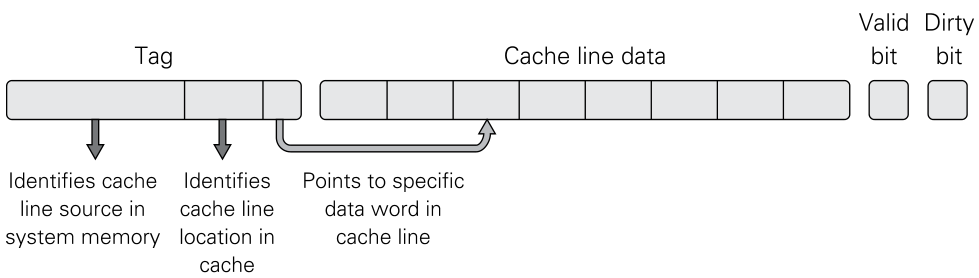
\includegraphics{images/performance/cache-line-structure.png}

}

\caption{\label{fig-performance-cache-line-structure}Struktur einer
Cache-Zeilen}

\end{figure}%

\subsection{GCC Optimization}\label{gcc-optimization}

\texttt{-O0} no optimization \texttt{-O3} all optimization
(\texttt{-O1},\texttt{-O2}) + function inlining and more

\texttt{funroll-loops}

\begin{tcolorbox}[enhanced jigsaw, toprule=.15mm, opacityback=0, colbacktitle=quarto-callout-tip-color!10!white, breakable, colframe=quarto-callout-tip-color-frame, title=\textcolor{quarto-callout-tip-color}{\faLightbulb}\hspace{0.5em}{Enabling Optimization}, left=2mm, arc=.35mm, toptitle=1mm, bottomrule=.15mm, rightrule=.15mm, titlerule=0mm, bottomtitle=1mm, leftrule=.75mm, opacitybacktitle=0.6, coltitle=black, colback=white]

\begin{Shaded}
\begin{Highlighting}[]
\PreprocessorTok{\#pragma GCC optimize ("O0")}
\end{Highlighting}
\end{Shaded}

\end{tcolorbox}

\subsection{}\label{section}

\newpage

\section{Safety}\label{safety}

\subsection{Terms}\label{terms}

\begin{description}
\tightlist
\item[Hazard]
A hazard is a situation in which there is actual or potential danger to
people or the environment.
\item[Accident]
An accident is an unintended event harming people or the environment.
\item[Incident]
An incident (or near miss) is an unintended event which does not harm,
but has the potential to do so.
\item[Risk]
To each hazard, the risk describes the likelihood of occurrence and the
likely consequences.
\item[Fault]
A fault is a defect within the system. Faults can be categorized into
random faults and systematic faults.
\item[Error]
An error is a deviation from the required operation of the system or
subsystem.
\item[System Failure]
A system failure occurs when the system fails to perform its required
function.
\item[Causalities]
The presence of a fault may lead to an error, which may lead to a system
failure, which may lead to an accident.
\end{description}

\subsection{Requirements}\label{requirements}


\includegraphics{images/safety/image-29.png}

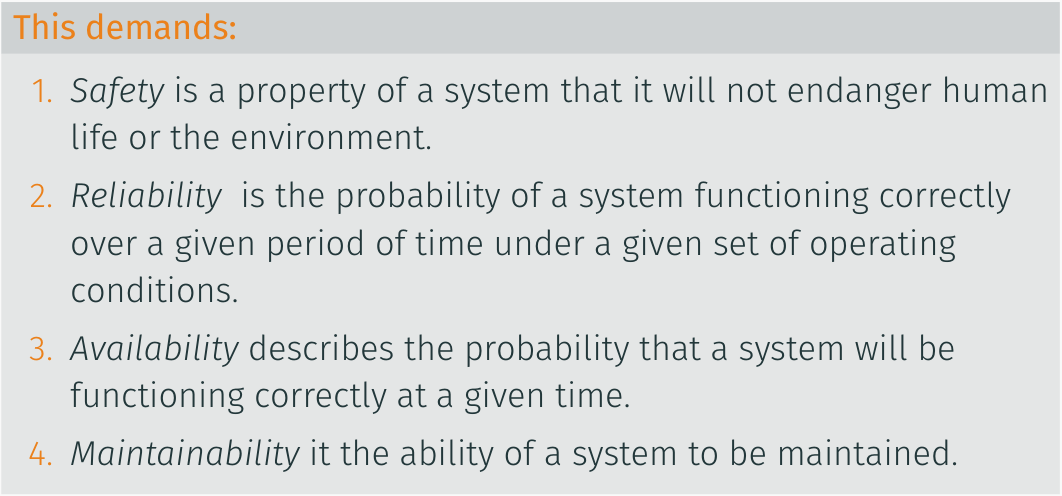
\includegraphics{images/safety/image-30.png}

\subsection{V\&V\&C}\label{vvc}

\begin{description}
\tightlist
\item[Verification]
Verification is the process of determining that a system, or module,
meets its specification.
\item[Validation]
Validation it the process of determining that a system is appropriate
for its purpose.
\item[Certification]
Certification it the process of convincing a regulatory bodies about a
systems properties.
\end{description}

\subsection{Computers in Safety Related
Systems?}\label{computers-in-safety-related-systems}

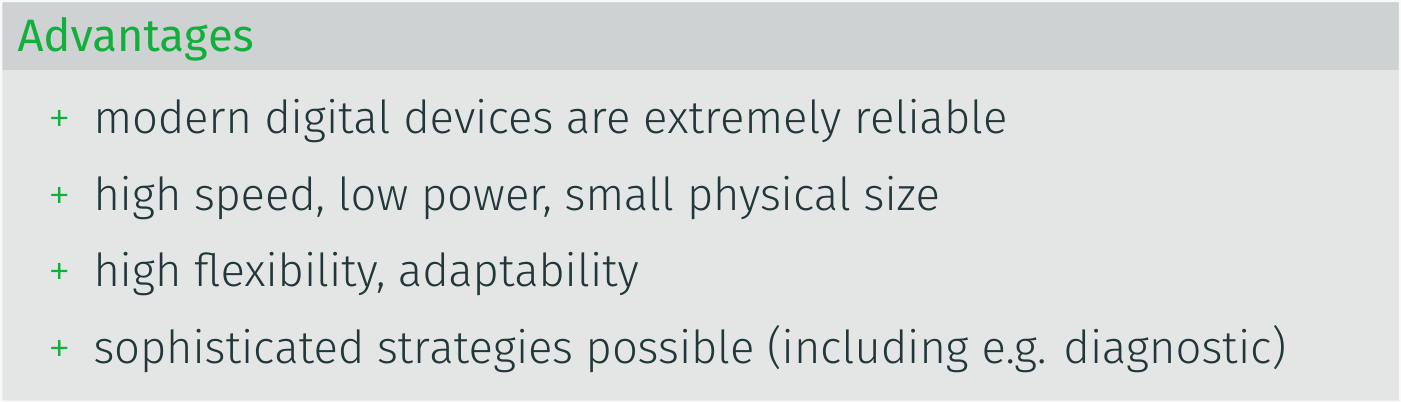
\includegraphics{images/safety/image-32.png}

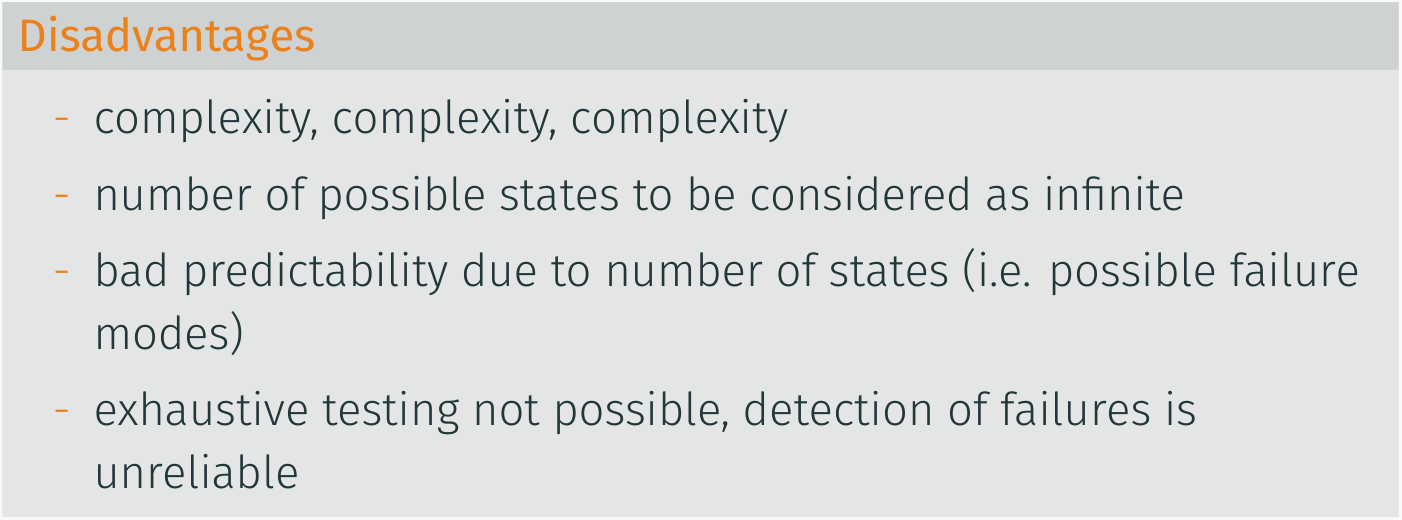
\includegraphics{images/safety/image-33.png}

\subsection{Silver Bullet}\label{silver-bullet}

There is good evidence that better processes lead to programs with fewer
defect. Some numbers in relation to the CMM (Capability Maturity Model)
level defined by Software Engineering Institute (SEI) according to:

\begin{center}
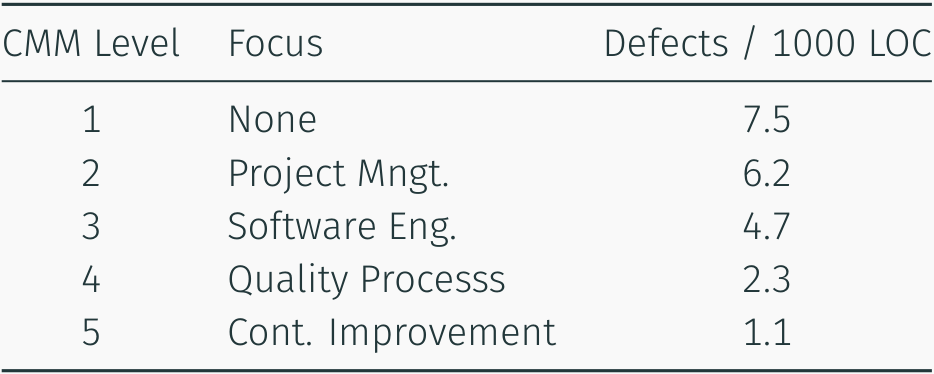
\includegraphics[width=\textwidth,height=4cm]{images/safety/image-31.png}
\end{center}

Brooks argues that \textbf{``there is no single development, in either
technology or management technique, which by itself promises even one
order of magnitude {[}tenfold{]} improvement within a decade in
productivity, in reliability, in simplicity.''} He also states that
\textbf{``we cannot expect ever to see two-fold gains every two years''}
in software development, as there is in hardware development (Moore's
law).

\subsection{Hazard Analysis}\label{hazard-analysis}

\vspace{-2mm}{\color{Orchid}\faQuestionCircle[regular]} \emph{How to
identify the ways in which a system can cause harm?}

\subsubsection{FMEA: Failure mode and effects
analysis}\label{fmea-failure-mode-and-effects-analysis}

Consider the failure of any component within a system and track the
effects of this failure to determine its ultimate consequences.

\subsubsection{HAZOP: Hazard and operability
studies}\label{hazop-hazard-and-operability-studies}

Use a series of 'guide words' to investigate the effects of deviations
from normal operating conditions.

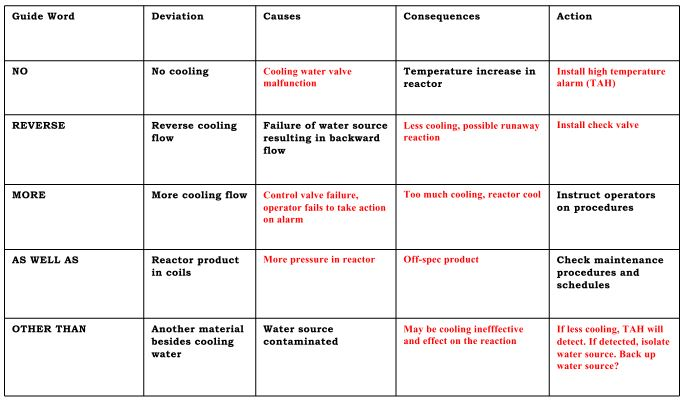
\includegraphics{images/safety/image.png}

\subsubsection{ETA: Event tree analysis}\label{eta-event-tree-analysis}

Take the events that can affect the system as starting point and track
them forward to determine their possible consequences.

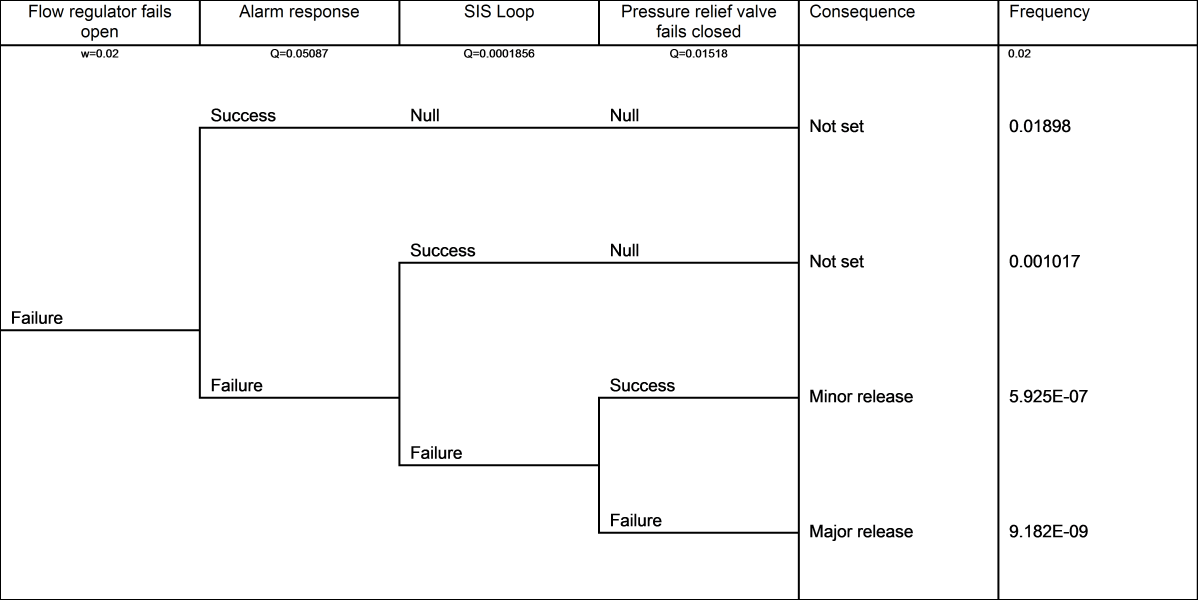
\includegraphics{images/safety/image-1.png}

\subsubsection{FTA: Fault tree analysis}\label{fta-fault-tree-analysis}

Start with all identified hazards and work backwards to determine their
possible causes. (Reverse to ETA)

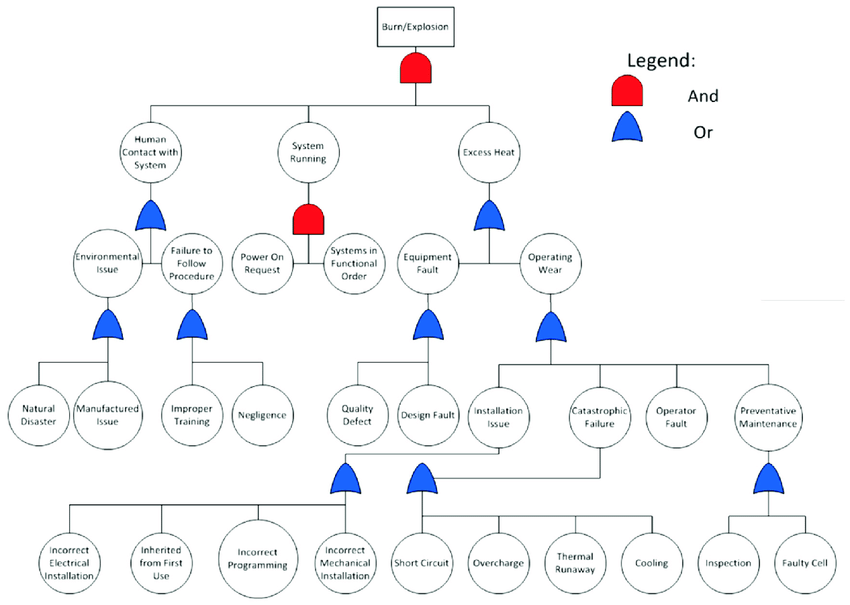
\includegraphics{images/safety/image-2.png}

\subsection{Risk Analysis}\label{risk-analysis}

\begin{tcolorbox}[enhanced jigsaw, toprule=.15mm, left=2mm, arc=.35mm, opacityback=0, rightrule=.15mm, breakable, bottomrule=.15mm, colframe=quarto-callout-important-color-frame, leftrule=.75mm, colback=white]
\begin{minipage}[t]{5.5mm}
\textcolor{quarto-callout-important-color}{\faExclamation}
\end{minipage}%
\begin{minipage}[t]{\textwidth - 5.5mm}

\vspace{-3mm}\textbf{Fundamental Rule}\vspace{3mm}

\[
\text{Risk} = \text{Severity} \times \text{Frequency} 
\]

\end{minipage}%
\end{tcolorbox}

\resizebox{\columnwidth}{!}{
  \begin{tikzpicture}[textbox/.style={font=\small, draw, text width=55, minimum height=40, inner sep=5, align=center}]
%text width
\node[textbox] (v1) at (-3.5,2.5) {Severity of hazardous event};
\node[textbox] (v3) at (-3.5,-1.5) {Frequency of hazardous event};
\node[textbox] (v2) at (-1,0.5) {Risk\\classification};
\node[textbox] (v4) at (2,0.5) {Integrity classification};
\node[textbox] (v5) at (4.5,2.5) {Hardware integrity classification};
\node[textbox] (v6) at (4.5,-1.5) {Systematic integrity classification};
\node[textbox] (v7) at (7.5,-1.5) {Software integrity classification};
\draw [-Latex] (v1) edge (v2);
\draw [-Latex] (v3) edge (v2);
\draw [-Latex] (v2) edge (v4);
\draw [-Latex] (v4) edge (v5);
\draw [-Latex] (v4) edge (v6);
\draw [-Latex] (v6) edge (v7);
\end{tikzpicture}
}

\begin{minipage}[c][1cm][c]{.7\columnwidth}

\subsubsection{Severity}\label{severity}

\vspace{-2mm}{\color{Orchid}\faQuestionCircle[regular]} \emph{How severe
is an accident?}

\end{minipage}%
\begin{minipage}[c][1cm][c]{.3\columnwidth}
\makebox[30mm][r]{
\resizebox{!}{0.9cm}{
  \begin{tikzpicture}[textbox/.style={font=\small, draw, minimum width=30, minimum height=20, inner sep=5, align=center}]
%text width
\node[textbox, fill=Orange!40] (v1) at (-2.5,1.5) {};
\node[textbox] (v3) at (-2.5,-0.5) {};
\node[textbox] (v2) at (-1.5,0.5) {};.
\node[textbox] (v4) at (0,0.5) {};
\node[textbox] (v5) at (1,1.5) {};
\node[textbox] (v6) at (1,-0.5) {};
\node[textbox] (v7) at (2.5,-0.5) {};
\draw [-Latex] (v1) edge (v2);
\draw [-Latex] (v3) edge (v2);
\draw [-Latex] (v2) edge (v4);
\draw [-Latex] (v4) edge (v5);
\draw [-Latex] (v4) edge (v6);
\draw [-Latex] (v6) edge (v7);
\end{tikzpicture}
}}
\end{minipage}

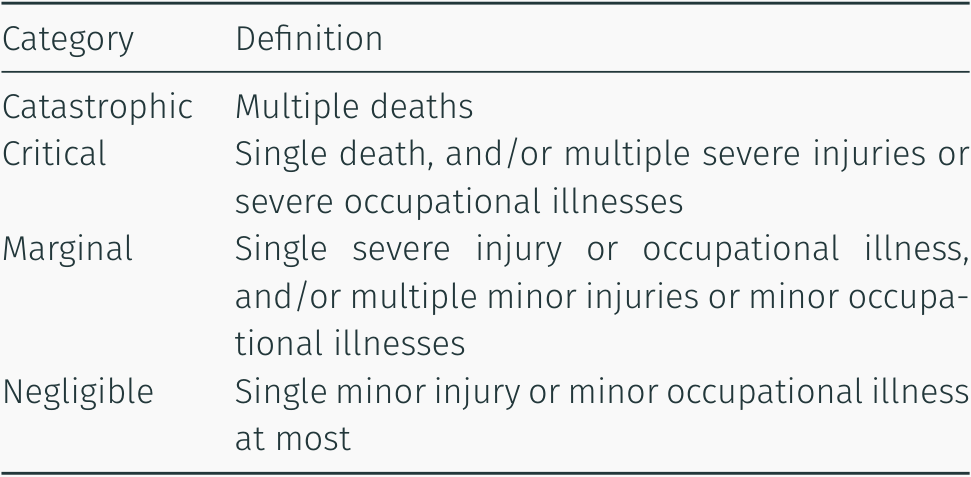
\includegraphics{images/safety/image-3.png}

\begin{minipage}[c][1cm][c]{.7\columnwidth}

\subsubsection{Frequency}\label{frequency}

\vspace{-2mm}{\color{Orchid}\faQuestionCircle[regular]} \emph{How
frequent does it occur?}

\end{minipage}%
\begin{minipage}[c][1cm][c]{.3\columnwidth}
\makebox[30mm][r]{
\resizebox{!}{0.9cm}{
  \begin{tikzpicture}[textbox/.style={font=\small, draw, minimum width=30, minimum height=20, inner sep=5, align=center}]
%text width
\node[textbox] (v1) at (-2.5,1.5) {};
\node[textbox, fill=Orange!40] (v3) at (-2.5,-0.5) {};
\node[textbox] (v2) at (-1.5,0.5) {};.
\node[textbox] (v4) at (0,0.5) {};
\node[textbox] (v5) at (1,1.5) {};
\node[textbox] (v6) at (1,-0.5) {};
\node[textbox] (v7) at (2.5,-0.5) {};
\draw [-Latex] (v1) edge (v2);
\draw [-Latex] (v3) edge (v2);
\draw [-Latex] (v2) edge (v4);
\draw [-Latex] (v4) edge (v5);
\draw [-Latex] (v4) edge (v6);
\draw [-Latex] (v6) edge (v7);
\end{tikzpicture}
}}
\end{minipage}

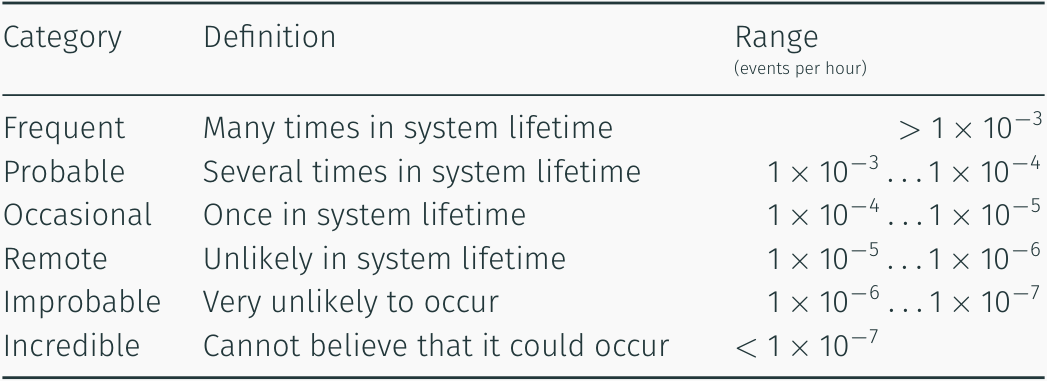
\includegraphics{images/safety/image-4.png}

\begin{minipage}[c][1cm][c]{.7\columnwidth}

\subsubsection{Risk}\label{risk}

\vspace{-2mm}{\color{Orchid}\faQuestionCircle[regular]} \emph{What is
the risk associated?}

\end{minipage}%
\begin{minipage}[c][1cm][c]{.3\columnwidth}
\makebox[30mm][r]{
\resizebox{!}{0.9cm}{
  \begin{tikzpicture}[textbox/.style={font=\small, draw, minimum width=30, minimum height=20, inner sep=5, align=center}]
%text width
\node[textbox] (v1) at (-2.5,1.5) {};
\node[textbox] (v3) at (-2.5,-0.5) {};
\node[textbox, fill=Orange!40] (v2) at (-1.5,0.5) {};.
\node[textbox] (v4) at (0,0.5) {};
\node[textbox] (v5) at (1,1.5) {};
\node[textbox] (v6) at (1,-0.5) {};
\node[textbox] (v7) at (2.5,-0.5) {};
\draw [-Latex] (v1) edge (v2);
\draw [-Latex] (v3) edge (v2);
\draw [-Latex] (v2) edge (v4);
\draw [-Latex] (v4) edge (v5);
\draw [-Latex] (v4) edge (v6);
\draw [-Latex] (v6) edge (v7);
\end{tikzpicture}
}}
\end{minipage}

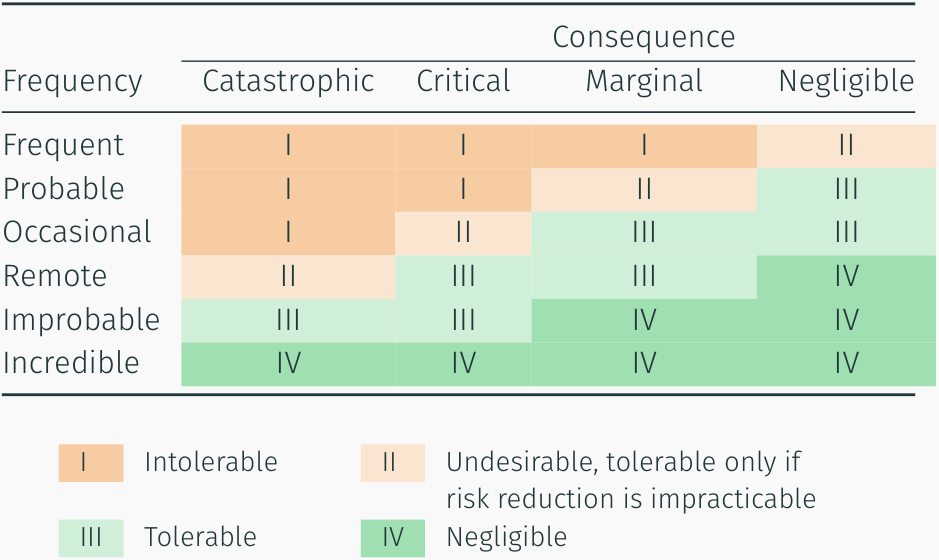
\includegraphics{images/safety/image-5.png}

\begin{minipage}[c][1cm][c]{.7\columnwidth}

\subsubsection{Integrity}\label{integrity}

\vspace{-2mm}{\color{Orchid}\faQuestionCircle[regular]} \emph{Is the
risk acceptable?}

\end{minipage}%
\begin{minipage}[c][1cm][c]{.3\columnwidth}
\makebox[30mm][r]{
\resizebox{!}{0.9cm}{
  \begin{tikzpicture}[textbox/.style={font=\small, draw, minimum width=30, minimum height=20, inner sep=5, align=center}]
%text width
\node[textbox] (v1) at (-2.5,1.5) {};
\node[textbox] (v3) at (-2.5,-0.5) {};
\node[textbox] (v2) at (-1.5,0.5) {};.
\node[textbox, fill=Orange!40] (v4) at (0,0.5) {};
\node[textbox] (v5) at (1,1.5) {};
\node[textbox] (v6) at (1,-0.5) {};
\node[textbox] (v7) at (2.5,-0.5) {};
\draw [-Latex] (v1) edge (v2);
\draw [-Latex] (v3) edge (v2);
\draw [-Latex] (v2) edge (v4);
\draw [-Latex] (v4) edge (v5);
\draw [-Latex] (v4) edge (v6);
\draw [-Latex] (v6) edge (v7);
\end{tikzpicture}
}}
\end{minipage}

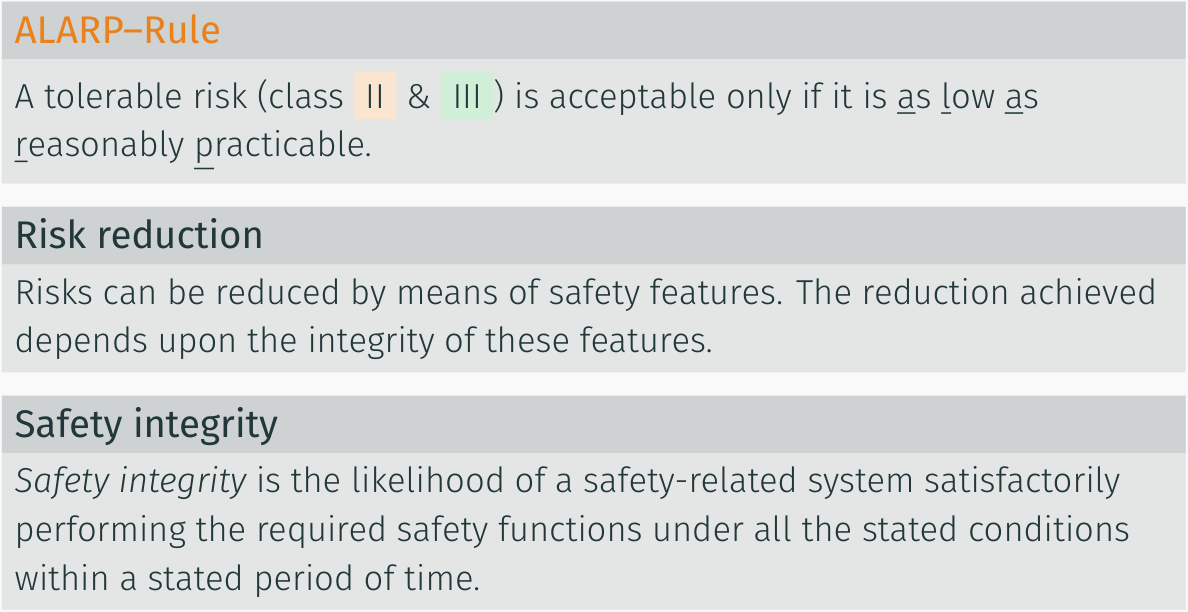
\includegraphics{images/safety/image-6.png}

\subsubsection{Integrity Levels}\label{integrity-levels}

\vspace{-2mm}{\color{Orchid}\faQuestionCircle[regular]} \emph{What
failure rate is tolerable?}

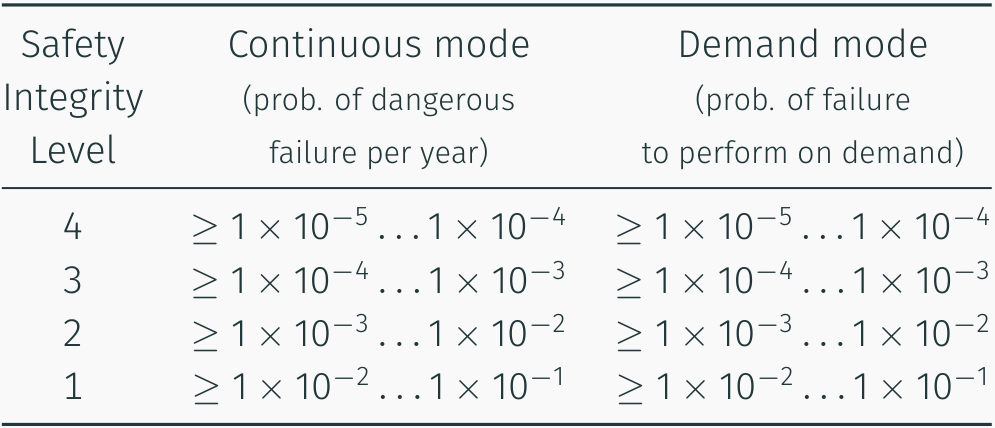
\includegraphics{images/safety/image-7.png}

\begin{tcolorbox}[enhanced jigsaw, toprule=.15mm, opacityback=0, colbacktitle=quarto-callout-tip-color!10!white, breakable, colframe=quarto-callout-tip-color-frame, title=\textcolor{quarto-callout-tip-color}{\faLightbulb}\hspace{0.5em}{Example -- Parachute}, left=2mm, arc=.35mm, toptitle=1mm, bottomrule=.15mm, rightrule=.15mm, titlerule=0mm, bottomtitle=1mm, leftrule=.75mm, opacitybacktitle=0.6, coltitle=black, colback=white]

{\small Hazard of free fall, severity rated as catastrophic with occasional frequency. Therefore risk is intolerable and a parachute is selected as safety feature. It works on demand mode and has to reduce the frequency by 2 orders of magnitudes, so SIL 2 is required at least.}

\end{tcolorbox}

\begin{tcolorbox}[enhanced jigsaw, toprule=.15mm, opacityback=0, colbacktitle=quarto-callout-important-color!10!white, breakable, colframe=quarto-callout-important-color-frame, title=\textcolor{quarto-callout-important-color}{\faExclamation}\hspace{0.5em}{Distinguish!}, left=2mm, arc=.35mm, toptitle=1mm, bottomrule=.15mm, rightrule=.15mm, titlerule=0mm, bottomtitle=1mm, leftrule=.75mm, opacitybacktitle=0.6, coltitle=black, colback=white]

{\bfseries\color{Orange}Risk} is a measure of the likelihood, and the
consequences, of a hazardous event.
{\bfseries\color{Orange}Safety integrity} is a measure of the likelihood
of the safety system correctly performing its task.

\end{tcolorbox}

\begin{minipage}[c][1cm][c]{.7\columnwidth}

\subsubsection{Allocating Levels}\label{allocating-levels}

\vspace{-2mm}{\color{Orchid}\faQuestionCircle[regular]} \emph{What is
contributing?}

\end{minipage}%
\begin{minipage}[c][1cm][c]{.3\columnwidth}
\makebox[30mm][r]{
\resizebox{!}{0.9cm}{
  \begin{tikzpicture}[textbox/.style={font=\small, draw, minimum width=30, minimum height=20, inner sep=5, align=center}]
%text width
\node[textbox] (v1) at (-2.5,1.5) {};
\node[textbox] (v3) at (-2.5,-0.5) {};
\node[textbox] (v2) at (-1.5,0.5) {};.
\node[textbox] (v4) at (0,0.5) {};
\node[textbox, fill=Orange!40] (v5) at (1,1.5) {};
\node[textbox, fill=Orange!40] (v6) at (1,-0.5) {};
\node[textbox, fill=Orange!40] (v7) at (2.5,-0.5) {};
\draw [-Latex] (v1) edge (v2);
\draw [-Latex] (v3) edge (v2);
\draw [-Latex] (v2) edge (v4);
\draw [-Latex] (v4) edge (v5);
\draw [-Latex] (v4) edge (v6);
\draw [-Latex] (v6) edge (v7);
\end{tikzpicture}
}}
\end{minipage}

\ul{Hardware} integrity is that part of the safety integrity relating to
dangerous \textbf{random} hardware failures.

\ul{Systematic} integrity is that part of the safety integrity relating
to dangerous \textbf{systematic} failures.

\ul{Software} integrity is that part of the safety integrity relating to
dangerous \textbf{software} failures.

\subsection{Design for Safety}\label{design-for-safety}

\begin{tcolorbox}[enhanced jigsaw, toprule=.15mm, opacityback=0, colbacktitle=quarto-callout-tip-color!10!white, breakable, colframe=quarto-callout-tip-color-frame, title=\textcolor{quarto-callout-tip-color}{\faLightbulb}\hspace{0.5em}{General, \ul{Iterative} Design Process}, left=2mm, arc=.35mm, toptitle=1mm, bottomrule=.15mm, rightrule=.15mm, titlerule=0mm, bottomtitle=1mm, leftrule=.75mm, opacitybacktitle=0.6, coltitle=black, colback=white]

\begin{enumerate}
\def\labelenumi{\arabic{enumi}.}
\tightlist
\item
  \textbf{Abstraction} Generlization \& ID of essentials
\item
  \textbf{Decomposition} Objects into smaller parts + Analysis
\item
  \textbf{Elaboration} detailing \& adding features
\item
  \textbf{Decision} identification \& selection of alternatives
\end{enumerate}

\end{tcolorbox}

\subsubsection{Types of Fault}\label{types-of-fault}

\vspace{-2mm}{\color{Orchid}\faQuestionCircle[regular]} \emph{What types
of fault may occure?}

\textHighlight{\bfseries N{\fontsize{7pt}{8pt}\selectfont{ATURE}}}

\begin{itemize}
\tightlist
\item
  Random (HW)
\item
  Systematic

  \begin{itemize}
  \tightlist
  \item
    Specification
  \item
    HW Design
  \item
    SW Design
  \end{itemize}
\end{itemize}

\textHighlight{\bfseries D{\fontsize{7pt}{8pt}\selectfont{URATION}}}

\begin{itemize}
\tightlist
\item
  Permanent -- most HW faults, design
\item
  Transient -- e.g.~\(\alpha\) particles
\item
  Intermittent -- e.g.~contacts, interference (EMC)
\end{itemize}

\textHighlight{\bfseries E{\fontsize{7pt}{8pt}\selectfont{XTEND}}}

\begin{itemize}
\tightlist
\item
  Localized -- affecting only part of the system
\item
  Global -- effects which permeate throughout the system
\end{itemize}

\subsection{Fault Tolerance}\label{fault-tolerance}

\subsubsection{Triple Modular Redundancy
(TMR)}\label{triple-modular-redundancy-tmr}

{\small\textit{Three identical moduls get fed by the same signal. A voter compares the results and produces an output corresponding to the majority view.}}

\begin{center}
\begin{tikzpicture}[
	textbox/.style={font=\small, draw, minimum width=30, minimum height=20, inner sep=5, align=center},
	circ/.style={circle, draw, minimum width=3, minimum height=3, inner sep=0, fill, align=center}
]
%text width
\node[textbox] (v1) at (-1,1) {Module 1};
\node[textbox] (v2) at (-1,0) {Module 2};
\node[textbox] (v4) at (-1,-1) {Module 3};
\node[textbox] (v5) at (1.5,0) {Voting\\element};
\node[circ] (v3) at (-2.5,0) {};
\draw  (v3) -- ++(-1.5,0) node[above right=-2] {\small Input};
\draw [-Latex, rounded corners] (v3) |- (v1);
\draw [-Latex, rounded corners] (v3) -- (v2);
\draw [-Latex, rounded corners] (v3) |- (v4);
\draw [-Latex] (v1) edge (v5);
\draw [-Latex] (v2) edge (v5);
\draw [-Latex] (v4) edge (v5);
\draw [-Latex] (v5) -- ++(2,0) node[above left=-2] {\small Output};
\end{tikzpicture}
\end{center}

{\small\begin{description}[parsep=0mm,labelsep=2pt,labelwidth=10pt]
  \item[\color{OliveGreen}\faPlus] simple
  \item[\color{OliveGreen}\faPlus] prevents from failure of a single component, i.e. \textit{single-point failure}
  \item[\color{BrickRed}\faMinus] leaves input and voter as sources for single-point failures
  \item[\color{BrickRed}\faMinus] does not prevent from systematic failures
  \item[\color{BrickRed}\faMinus] voter is dependable
\end{description}}

\subsubsection{Voter}\label{voter}

{\small\textit{To make voting unit reliable, keep it as simple as possible.}}

\begin{center}
\begin{tikzpicture}[
	textbox/.style={font=\small, draw, minimum width=5mm, minimum height=5mm, inner sep=0, align=center},
	circ/.style={circle, draw, minimum width=3, minimum height=3, inner sep=0, fill, align=center}
]
%text width
\node[textbox] (v1) at (-0.5,1) {\&};
\node[textbox] (v2) at (-0.5,0) {\&};
\node[textbox] (v3) at (-0.5,-1) {\&};
\node[textbox] (v5) at (1.5,0) {\&};

\node[circ] (dot1) at (-1.5,1.125) {};
\draw  (dot1) -- ++(-1.75,0) node[above right=-2] {\small Input 1};
\node[circ] (dot2) at (-1.25,0.125) {};
\draw  (dot2) -- ++(-2,0) node[above right=-2] {\small Input 2};
\node[circ] (dot3) at (-1,-0.875) {};
\draw  (dot3) -- ++(-2.25,0) node[above right=-2] {\small Input 3};


\draw [{Circle[open]}-] (v5) -- ++(2,0) node[above left=-2] {\small Output};
\node (v4) at (-0.75,1.125) {};
\node (v10) at (-0.75,0.875) {};
\node (v8) at (-0.75,0.125) {};
\node (v9) at (-0.75,-0.125) {};
\node (v7) at (-0.75,-0.875) {};
\node (v6) at (-0.75,-1.125) {};
\node (v11) at (1.25,0.15) {};
\node (v12) at (1.25,0) {};
\node (v13) at (1.25,-0.15) {};
\node (info) at (2,1) {\bfseries (example)};
\draw  (dot1) |- (v4.center);
\draw  (dot1) |- (v6.center);
\draw  (dot3) |- (v7.center);
\draw  (dot2) |- (v8.center);
\draw  (dot3) |- (v9.center);
\draw  (dot2) |- (v10.center);
\draw [{Circle[open]}-Latex] (v1) -| ++(1,0) |-  (v11.center);
\draw [{Circle[open]}-Latex] (v2) edge (v12.center);
\draw [{Circle[open]}-Latex] (v3) -| ++(1,0) |- (v13.center);
\end{tikzpicture}
\end{center}

{\small\begin{description}[parsep=0mm,labelsep=2pt,labelwidth=10pt]
  \item[\color{OliveGreen}\faPlus] simple, low complexity
  \item[\color{OliveGreen}\faPlus] high reliability
  \item[\color{BrickRed}\faMinus] no indication in case of discrepancies
\end{description}}

\subsubsection{TMR with triple voting}\label{tmr-with-triple-voting}

{\small\textit{Use triple input signals and triple voting instances.}}

\begin{center}
\begin{tikzpicture}[
	textbox/.style={font=\small, draw, text width=40, minimum height=25, inner sep=3, align=center},
	circ/.style={circle, draw, minimum width=3, minimum height=3, inner sep=0, fill, align=center}
]
\node[textbox] (mod1) at (0, 1) {Module 1};
\node[textbox] (mod2) at (0, 0) {Module 2};
\node[textbox] (mod3) at (0,-1) {Module 3};

\node[textbox] (vote1) at (3, 1) {Voting\\element};
\node[textbox] (vote2) at (3, 0) {Voting\\element};
\node[textbox] (vote3) at (3,-1) {Voting\\element};
\draw[-Latex]  (mod1.east) -- (vote1.west);
\draw[-Latex]  (mod1.east) -- ([yshift=3]vote2.west);
\draw[-Latex]  (mod1.east) -- ([yshift=8]vote3.west);
\draw[-Latex]  (mod2.east) -- ([yshift=-3]vote1.west);
\draw[-Latex]  (mod2.east) -- (vote2.west);
\draw[-Latex]  (mod2.east) -- ([yshift=3]vote3.west);
\draw[-Latex]  (mod3.east) -- ([yshift=-8]vote1.west);
\draw[-Latex]  (mod3.east) -- ([yshift=-3]vote2.west);
\draw[-Latex]  (mod3.east) -- (vote3.west);

\draw[Latex-]  (mod1) -- ++(-2.5,0) node[above right=-2] {\small Input 1};
\draw[Latex-]  (mod2) -- ++(-2.5,0) node[above right=-2] {\small Input 2};
\draw[Latex-]  (mod3) -- ++(-2.5,0) node[above right=-2] {\small Input 3};

\draw[-Latex]  (vote1) -- ++(2.5,0) node[above left=-2] {\small Output 1};
\draw[-Latex]  (vote2) -- ++(2.5,0) node[above left=-2] {\small Output 2};
\draw[-Latex]  (vote3) -- ++(2.5,0) node[above left=-2] {\small Output 3};
\end{tikzpicture}
\end{center}

{\small\begin{description}[parsep=0mm,labelsep=2pt,labelwidth=10pt]
  \item[\color{OliveGreen}\faPlus] \textbf{all} outputs are correct in case a single module fails
  \item[\color{BrickRed}\faMinus] more components required
  \item[\color{BrickRed}\faMinus] no protection against simultaneous failure of two or more modules
  \item[\color{BrickRed}\faMinus] does not prevent from systematic failures
\end{description}}

\subsubsection{Multistage TMR}\label{multistage-tmr}

{\small\textit{Cascading TMRs with triple voters can deal with failed voting unit.}}

\resizebox{\columnwidth}{!}{
\begin{tikzpicture}[
	textbox/.style={font=\scriptsize, draw, text width=30, minimum height=20, inner sep=3, align=center},
	circ/.style={circle, draw, minimum width=3, minimum height=3, inner sep=0, fill, align=center}
]
\node[textbox] (mod11) at (0, 1) {Module};
\node[textbox] (mod12) at (0, 0) {Module};
\node[textbox] (mod13) at (0,-1) {Module};

\node[textbox] (vote11) at (2.5, 1) {Voting\\element};
\node[textbox] (vote12) at (2.5, 0) {Voting\\element};
\node[textbox] (vote13) at (2.5,-1) {Voting\\element};

\draw[-Latex]  (mod11.east) -- (vote11.west);
\draw[-Latex]  (mod11.east) -- ([yshift=3]vote12.west);
\draw[-Latex]  (mod11.east) -- ([yshift=8]vote13.west);
\draw[-Latex]  (mod12.east) -- ([yshift=-3]vote11.west);
\draw[-Latex]  (mod12.east) -- (vote12.west);
\draw[-Latex]  (mod12.east) -- ([yshift=3]vote13.west);
\draw[-Latex]  (mod13.east) -- ([yshift=-8]vote11.west);
\draw[-Latex]  (mod13.east) -- ([yshift=-3]vote12.west);
\draw[-Latex]  (mod13.east) -- (vote13.west);
	
\draw[Latex-]  (mod11) -- ++(-2,0) node[above right=-2] {\footnotesize Input 1};
\draw[Latex-]  (mod12) -- ++(-2,0) node[above right=-2] {\footnotesize Input 2};
\draw[Latex-]  (mod13) -- ++(-2,0) node[above right=-2] {\footnotesize Input 3};

\node[textbox] (mod21) at (4.5,1) {Module};
\node[textbox] (mod22) at (4.5,0) {Module};
\node[textbox] (mod23) at (4.5,-1) {Module};

\node[textbox] (vote21) at (7,1) {Voting\\element};
\node[textbox] (vote22) at (7,0) {Voting\\element};
\node[textbox] (vote23) at (7,-1) {Voting\\element};

\draw [-Latex] (vote11) -- (mod21);
\draw [-Latex] (vote12) -- (mod22);
\draw [-Latex] (vote13) -- (mod23);
\draw [-Latex] (mod21.east) -- (vote21.west);
\draw [-Latex] (mod21.east) -- ([yshift=3]vote22.west);
\draw [-Latex] (mod21.east) -- ([yshift=8]vote23.west);
\draw [-Latex] (mod22.east) -- ([yshift=-3]vote21.west);
\draw [-Latex] (mod22.east) -- (vote22.west);
\draw [-Latex] (mod22.east) -- ([yshift=3]vote23.west);
\draw [-Latex] (mod23.east) -- (vote23.west);
\draw [-Latex] (mod23.east) -- ([yshift=-3]vote22.west);
\draw [-Latex] (mod23.east) -- ([yshift=-8]vote21.west);

\draw[-Latex]  (vote21) -- ++(2,0) node[above left=-2] {\footnotesize Output 1};
\draw[-Latex]  (vote22) -- ++(2,0) node[above left=-2] {\footnotesize Output 2};
\draw[-Latex]  (vote23) -- ++(2,0) node[above left=-2] {\footnotesize Output 3};
\end{tikzpicture}}

{\small\begin{description}[parsep=0mm,labelsep=2pt,labelwidth=10pt]
  \item[\color{OliveGreen}\faPlus] allows a single module to fail at each level
  \item[\color{OliveGreen}\faPlus] allows a single voter to fail at each level
  \item[\color{BrickRed}\faMinus] no protection against simultaneous failure of two or more units at same level
  \item[\color{BrickRed}\faMinus] does not prevent from systematic failure
\end{description}}

\subsubsection{\texorpdfstring{NMR - \(N\) Modular
Redundancy}{NMR - N Modular Redundancy}}\label{nmr---n-modular-redundancy}

{\small\textit{Use a large (odd) number of modules to increase ability to withstand failures.}}

\begin{center}
\begin{tikzpicture}[
	textbox/.style={font=\small, draw, text width=40, minimum height=25, inner sep=3, align=center},
	circ/.style={circle, draw, minimum width=2, minimum height=2, inner sep=0, fill, align=center}
]
\node[textbox] (mod1) at (0, 1) {Module 1};
\node[textbox] (mod2) at (0, 0) {Module 2};
\node[textbox] (mod3) at (0,-2) {Module N};
\node[circ] at (0,-0.75) {};
\node[circ] at (0,-1) {};
\node[circ] at (0,-1.25) {};

\node[textbox] (vote) at (3,-0.5) {Voting\\element};

\draw[Latex-]  (mod1) -- ++(-2.5,0) node[above right=-2] {\small Input 1};
\draw[Latex-]  (mod2) -- ++(-2.5,0) node[above right=-2] {\small Input 2};
\draw[Latex-]  (mod3) -- ++(-2.5,0) node[above right=-2] {\small Input N};

\draw[-Latex]  (vote) -- ++(2.5,0) node[above left=-2] {\small Output};
\draw[-Latex]  (mod2.east) -- (vote.west);
\draw[-Latex]  (mod1.east) -- ([yshift=5]vote.west);
\draw[-Latex]  (mod3.east) -- ([yshift=-5]vote.west);
\end{tikzpicture}
\end{center}

{\small\begin{description}[parsep=0mm,labelsep=2pt,labelwidth=10pt]
  \item[\color{OliveGreen}\faPlus] allows  $\sfrac{(N-1)}{2}$ modules to fail
  \item[\color{BrickRed}\faMinus] higher complexity of voter
  \item[\color{BrickRed}\faMinus] higher cost, size, power consumption
\end{description}}

\subsubsection{Dynamic Redundancy}\label{dynamic-redundancy}

{\small\textit{While no fault is detected, one module drives the output. In case of a fault, a switch reconfigures the system such that the output is taken from a ’standby spare’ module.}}

\begin{center}
\begin{tikzpicture}[
	textbox/.style={font=\small, draw, text width=40, minimum height=25, inner ysep=0, align=center},
	circ/.style={circle, draw, minimum width=3, minimum height=3, inner sep=0, fill, align=center}
]
\node[textbox] (mod1) at (0, 1) {Module 1};
\node[textbox] (mod2) at (0, 0) {Module 2};
\node[textbox] (fault) at (1.75,2.25) {Fault\\detector};
\node[textbox, minimum height=55, text width=30] (switch) at (3.5,0.5) {Switch};

\node [circ] (v3) at (-1.25,0.5) {};

\draw[-]  (v3) -- ++(-1.25,0) node[above right=-2] {\small Input};
\draw[-Latex]  (switch) -- ++(2,0) node[above left=-2] {\small Output};

\draw[-Latex]  (mod1.east) -- (switch.west |- mod1);
\draw[-Latex]  (mod2.east) -- (switch.west |- mod2);
\node [circ] (v1) at (2.15,1) {};
\node [circ] (v2) at (1.35,0) {};
\draw [-Latex] (v1) -- (fault.south -| v1);
\draw [-Latex] (v2) -- (fault.south -| v2);
\draw [-Latex,rounded corners] (fault) -| (switch);
\draw [-Latex,rounded corners] (v3) |- (mod1);
\draw [-Latex,rounded corners] (v3) |- (mod2);
\end{tikzpicture}
\end{center}

{\small\begin{description}[parsep=0mm,labelsep=2pt,labelwidth=10pt]
  \item[\color{OliveGreen}\faPlus] allows one modules to fail
  \item[\color{OliveGreen}\faPlus] gives indication of fault
  \item[\color{BrickRed}\faMinus] fault detector required (single-point failure!)
  \item[\color{Orange}\bfseries ±] either \textit{hot standby} or \textit{cold standby} possible
  \item[\color{Orange}\bfseries ±] can be extended to $N$ modules
\end{description}}

\subsubsection{Self Checking Pair}\label{self-checking-pair}

{\small\textit{The output of two identical modules are compared to give an indication of failure.}}

\begin{center}
\begin{tikzpicture}[
	textbox/.style={font=\small, draw, minimum width=40, minimum height=20, inner ysep=0, align=center},
	circ/.style={circle, draw, minimum width=3, minimum height=3, inner sep=0, fill, align=center}
]
\node[textbox] (mod1) at (0,1.5) {Module 1};
\node[textbox] (mod2) at (0,-0.5) {Module 2};
\node[textbox] (switch) at (2.75,-0.25) {Comparator};

\node [circ] (v3) at (-1.25,0.5) {};

\draw[-]  (v3) -- ++(-1.25,0) node[above right=-2] {\small Input};
\draw[-Latex]  (switch) -- ++(2.25,0) node[above left=-1] {\small Failure};

\draw[-Latex]  (mod1.east) -- ++(4.25,0)  node[above left=-1] {\small Output};
\draw[-Latex]  (mod2.east) -- (switch.west |- mod2);
\node [circ] (v1) at (1.25,1.5) {};
\draw [-Latex,rounded corners] (v3) |- (mod1);
\draw [-Latex,rounded corners] (v3) |- (mod2);
\node (v2) at (1.25,0) {};
\draw [-Latex,rounded corners] (v1) -- (v2.center) -- (switch.west |- v2);
\end{tikzpicture}
\end{center}

{\small\begin{description}[parsep=0mm,labelsep=2pt,labelwidth=10pt]
  \item[\color{OliveGreen}\faPlus] simple, reliable
  \item[\color{OliveGreen}\faPlus] gives indication of fault
  \item[\color{BrickRed}\faMinus] no redundancy
\end{description}}

\subsubsection{Redundancy Combining}\label{redundancy-combining}

{\small\begin{description}[style=sameline,parsep=0mm,labelsep=2pt,labelwidth=10pt]
  \item[\textHighlight{\bfseries S{\fontsize{6.5pt}{7pt}\selectfont{TATIC}}}] Voting to produce \textit{fault masking} at the cost of large amount of redundancy.
  \item[\textHighlight{\bfseries D{\fontsize{6.5pt}{7pt}\selectfont{YNAMIC}}}] Fault detection and some form of switching, but \textbf{do not} mask faults.
  \item[\textHighlight{\bfseries H{\fontsize{6.5pt}{7pt}\selectfont{YBRID}}}] Combination of voting, fault detection and module switching $\rightarrow$ Most reduced down to \textit{N-modular redundancy with spares}.
\end{description}}

\subsubsection{Software Faults}\label{software-faults}

{\small\textit{Software faults are systematic by nature, duplicating the systems gives therefore no protection from faults.}}

{\small\begin{description}[style=sameline,parsep=0mm,labelsep=2pt,labelwidth=10pt]
  \item[\textHighlight{\bfseries $\mathbf{N}$-Version Programming}] Same function gets implemented differently with the same specifications. ($N=3$ for Airbus, $N=4$ for Space Shuttle)
  \item[\textHighlight{\bfseries Recovery Blocks}] When a module fails, it induces (triggers) the execution of a secondary implementation of the same module.
\end{description}}

\subsection{Reliability}\label{reliability}

\subsubsection{\texorpdfstring{(Un)-Reliability \(R\)
(\(Q\))}{(Un)-Reliability R (Q)}}\label{un-reliability-r-q}

Reliability \(R\) is the probability of a component/system functioning
correctly over a given period of time and a given set of operating
condition.

\[
R(t)=\frac{n(t)}{N}
\]

\begin{conditions*}
  N & Amount of identical components \\
  n(t) & expected number of components operating correctly at some time $t$
\end{conditions*}

The \textbf{un}reliability \(Q\) defines how likely it is that the
system/component will break.

\[
Q(t)=\frac{n_f(t)}{N}=1-R(t)
\]

\begin{conditions*}
  n_f(t) & expected number of malfunctioning components at some time $t$.
\end{conditions*}

\subsubsection{\texorpdfstring{Failure Rate
\(z(t)\)}{Failure Rate z(t)}}\label{failure-rate-zt}

Is the rate at which a device fails. Number of devices failing within a
given period of time as a fraction of the devices still functioning.

\[
z(t)=\frac{1}{n(t)}\cdot\frac{d~n_f(t)}{dt}
\]

\subsubsection{Bathtub Curve}\label{bathtub-curve}

\begin{center}
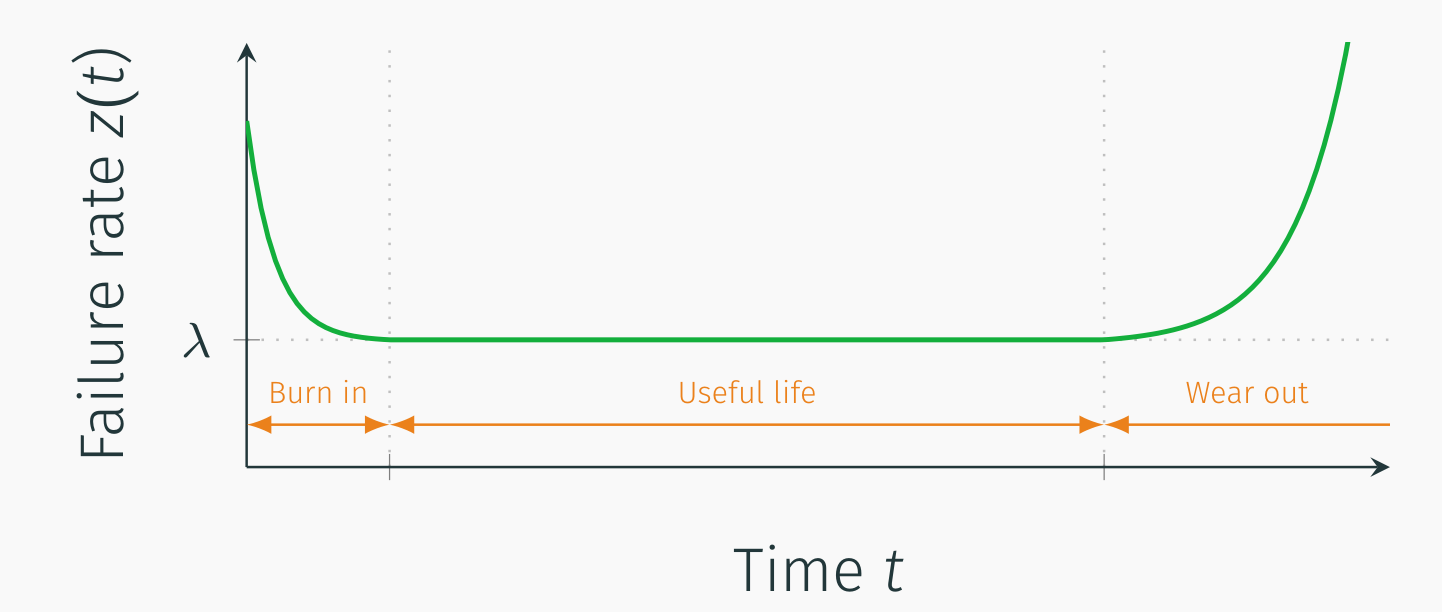
\includegraphics[width=6cm,height=\textheight]{images/safety/image-10.png}
\end{center}

{\small\begin{description}[style=sameline,parsep=0mm,labelsep=2pt,labelwidth=10pt]
  \item[\textbf{Burn in}] high ’infant mortality’ due to manufacturing faults.
  \item[\textbf{Useful life}]  the failure rate takes in a fairly constant level $\lambda$.
  \item[\textbf{Wear out}] ageing becomes apart and the failure rate rises.
\end{description}}

\subsubsection{Useful-Life}\label{useful-life}

If the failure rate is constant, \(z(t)=\lambda\),

\[
z(t)=\lambda=\frac{1}{n(t)}\cdot\frac{d~n_f(t)}{dt}
\]

with \(n_f(t) = N - n(t)\) we get the differential equation

\[
\lambda n(t) = \frac{dN-n}{dt}=-\frac{dt}{dt}
\]

with solution for \(R(t) = \sfrac{n(t)}{N}\)

\[
R(t)=\exp(-\lambda\cdot t)
\]

\subsubsection{Time-Variant Failure
Rates}\label{time-variant-failure-rates}

For software failures, which are systematic and therefore correctable
after detection, the failure rate decreases with time. The reliability
resulting can by modelled by the \emph{Weibull} distribution:

\[
R(t)=\exp(-(\sfrac{t}{\eta})^\beta)
\]

\begin{conditions*}
  \beta & shape parameter\\
  \eta & characteristic life
\end{conditions*}

\subsection{Mean times}\label{mean-times}

\subsubsection{Mean Time to Failure}\label{mean-time-to-failure}

\vspace{-2mm}{\color{Orchid}\faQuestionCircle[regular]} \emph{What is
the expected time that a system will operate before the first failure
occures?}

\[
MTTF=\int_0^\infty R(t)~dt\rightarrow\int_0^\infty \exp(-\lambda\cdot t)~dt=\frac{1}{\lambda}
\]

\begin{tcolorbox}[enhanced jigsaw, toprule=.15mm, opacityback=0, colbacktitle=quarto-callout-caution-color!10!white, breakable, colframe=quarto-callout-caution-color-frame, title=\textcolor{quarto-callout-caution-color}{\faFire}\hspace{0.5em}{Beware!}, left=2mm, arc=.35mm, toptitle=1mm, bottomrule=.15mm, rightrule=.15mm, titlerule=0mm, bottomtitle=1mm, leftrule=.75mm, opacitybacktitle=0.6, coltitle=black, colback=white]

{\small A system with $\lambda=0.001$ failure/h does have a MTTF of $1000$ hour. But the reliability at t = 1000 hour is $R(t)=e^{-\lambda\cdot t}=e^{-1}\approx 0.37$. Chances that any given system runs for 1000 hour are only $\approx37\%$!}

\end{tcolorbox}

\begin{tcolorbox}[enhanced jigsaw, toprule=.15mm, opacityback=0, colbacktitle=quarto-callout-important-color!10!white, breakable, colframe=quarto-callout-important-color-frame, title=\textcolor{quarto-callout-important-color}{\faExclamation}\hspace{0.5em}{Reliability vs.~MTTF}, left=2mm, arc=.35mm, toptitle=1mm, bottomrule=.15mm, rightrule=.15mm, titlerule=0mm, bottomtitle=1mm, leftrule=.75mm, opacitybacktitle=0.6, coltitle=black, colback=white]

\begin{description}
\tightlist
\item[Reliability]
a function of time, depends on the time for which the system must
operate.
\item[MTTF]
fixed characteristic that does not change with time.
\end{description}

\end{tcolorbox}

\subsubsection{Mean Time to Repair}\label{mean-time-to-repair}

\vspace{-2mm}{\color{Orchid}\faQuestionCircle[regular]} \emph{What is
the average time required to repair a system that has failed?}

\[
MTTR=\frac{1}{\mu}\qquad MTBF=MTTF + MTTR
\]

\begin{conditions*}
  MTTR & Mean time to repair\\
  MTBF & Mean time between failures
\end{conditions*}

\subsection{Failure in time}\label{failure-in-time}

\vspace{-2mm}{\color{Orchid}\faQuestionCircle[regular]} \emph{How many
failures are to be expected?}

Failure in time (FIT) is the number of failures that can be expected in
\(1\times 10^9\) h of operation.

\[
FIT = 1\times 10^9\cdot\frac{1}{MTBF}
\]

\subsection{Reliability modelling}\label{reliability-modelling}

\begin{center}
\begin{tikzpicture}[
	textbox/.style={font=\small, draw, text width=20, minimum height=20, inner sep=0, align=center},
	circ/.style={circle, draw, minimum width=2, minimum height=2, inner sep=0, fill, align=center}
]
\node[textbox] (b1) at (0, 0) {1};
\node[textbox] (b2) at (1.5, 0) {2};
\node[textbox] (b3) at (4.5, 0) {N};

\draw[Latex-] (b1) -- ++(-1.5,0) node[above right=-1] {\small Input};
\draw[-Latex] (b3) -- ++(1.5,0) node[above left=-1] {\small Output};
\draw[-] (b2) -- ++(1,0) ;
\draw[-,dashed] (b2) ++(1,0) -- ++(1,0);
\draw[-] (b2) ++(2,0) -- (b3);
\draw[-Latex] (b3) -- ++(1.5,0) node[above left=-1] {\small Output};

\draw [-Latex] (b1) edge (b2);
\end{tikzpicture}
\end{center}

\[
R(t)=R_1(t)\cdot R_2(t)\cdot\cdots\cdot R_N(t)=\prod_{i=1}^N R_i(t)
\]

\[
\lambda=\lambda_1+\lambda_2+\cdots=\sum_{i=1}^N \lambda_i
\]

\begin{center}
\begin{tikzpicture}[
	textbox/.style={font=\small, draw, text width=20, minimum height=20, inner sep=0, align=center},
	circ/.style={circle, draw, minimum width=3, minimum height=3, inner sep=0, fill, align=center}
]
\node[textbox] (b1) at (1,1) {1};
\node[textbox] (b2) at (1,0) {2};
\node[textbox] (b3) at (1,-1.5) {N};
\node [circ] (dot1) at (0,0) {};
\node [circ] (dot2) at (2,0) {};

\draw[-] (dot1) -- ++(-1.5,0) node[above right=-1] {\small Input};
\draw[-Latex] (dot2) -- ++(1.5,0) node[above left=-1] {\small Output};


\draw [-Latex] (dot1) |- (b1);
\draw [-Latex] (dot1) |- (b2);
\draw [-Latex] (dot1) |- (b3);
\draw [-] (b3) -| (dot2);
\draw [-] (b2) -| (dot2);
\draw [-] (b1) -| (dot2);
\node[circ, minimum width=2, minimum height=2] at (1,-0.65) {};
\node[circ, minimum width=2, minimum height=2] at (1,-0.85) {};
\end{tikzpicture}
\end{center}

\[
R(t)=1-Q(t)=1-\prod_{i=1}^N(1-R_i(t))
\]

\[
Q(t)=Q_1(t)\cdot Q_2(t)\cdots Q_N(t)=\prod_{i=1}^N Q_i(t)
\]

\subsubsection{Triple Modular
Redundancy}\label{triple-modular-redundancy}

\begin{center}
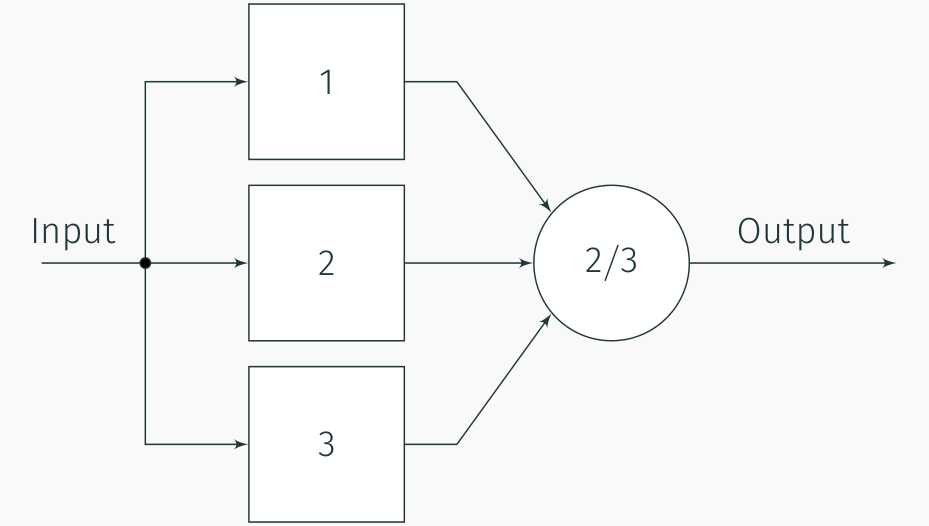
\includegraphics[width=\textwidth,height=4cm]{images/safety/image-11.png}
\end{center}

\[
\begin{split}
R_{TMR}=R_1(t)\cdot R_2(t)\cdot R_3(t) &+ (1-R_1(t))\cdot R_2(t)\cdot R_3(t)\\
                                       &+ (1-R_2(t))\cdot R_1(t)\cdot R_3(t)\\
                                       &+ (1-R_3(t))\cdot R_1(t)\cdot R_2(t)\\
\end{split}
\]

For \(R_1=R_2=R_3=R_m\): \(R(t)=3\cdot R_m^2(t)-2\cdot R_m^3(t)\)

\begin{tcolorbox}[enhanced jigsaw, toprule=.15mm, opacityback=0, colbacktitle=quarto-callout-important-color!10!white, breakable, colframe=quarto-callout-important-color-frame, title=\textcolor{quarto-callout-important-color}{\faExclamation}\hspace{0.5em}{N-Modular Redundancy}, left=2mm, arc=.35mm, toptitle=1mm, bottomrule=.15mm, rightrule=.15mm, titlerule=0mm, bottomtitle=1mm, leftrule=.75mm, opacitybacktitle=0.6, coltitle=black, colback=white]

{\bfseries\color{Orange}M out of N voting}: System works correctly as
long as {\bfseries\color{Orange}less then M} modules fail.

\begin{center}
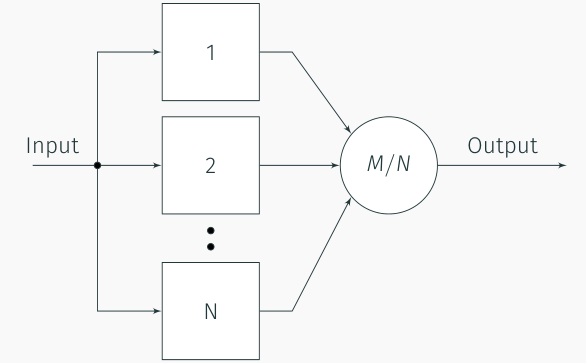
\includegraphics[width=\textwidth,height=4cm]{images/safety/image-12.png}
\end{center}

\[
R_{MtoN}(t)=\sum_{i=0}^{N-M}\frac{N!}{(N-i)!\cdot i!}\cdot R_m^{N-i}(t)\cdot (1-R_m(t))^i
\]

\end{tcolorbox}

\subsubsection{Dynamic Redundancy}\label{dynamic-redundancy-1}

\begin{center}
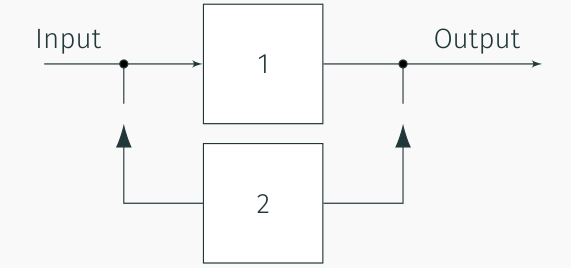
\includegraphics[width=\textwidth,height=3cm]{images/safety/image-13.png}
\end{center}

\[
\begin{split}
R(t)&=R_1(t)+(1-R_1(t))\cdot C_1\cdot R_2(t)\\
    &=R_m(t)+(1-R_m(t))\cdot C_m\cdot R_m(t)
\end{split}
\]

\begin{conditions*}
  R_n & Module Probabilities\\
  C_n & Fault Coverage
\end{conditions*}

\subsubsection{Cut and Tie Sets}\label{cut-and-tie-sets}

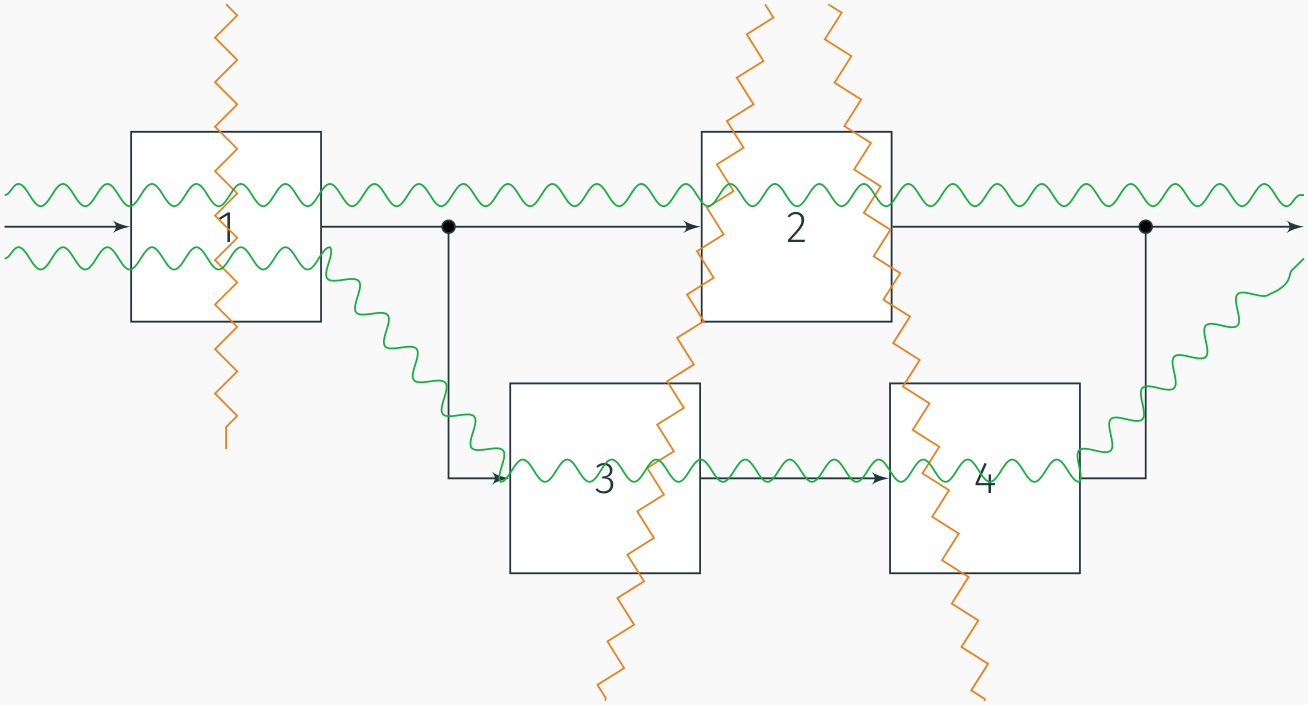
\includegraphics{images/safety/image-14.png}

\begin{conditions*}
  {\color{Orange}\rightsquigarrow\textbf{ cut}} & sets of simultaneous failures leading to a system failure\\
  {\color{OliveGreen}\rightsquigarrow\textbf{ tie}} & sets of working modules guaranteeing a working system
\end{conditions*}

\[
1-\sum_{j=1}^{\textcolor{Orange}{\mathbf{N_C}}}\prod_{i=1}^{n_j}(1-R_i(t))\leq R(t) \leq \sum_{j=1}^{\textcolor{OliveGreen}{\mathbf{N_T}}}\prod_{i=1}^{n_j}(1-R_i(t))
\]

\subsection{Reliability prediction}\label{reliability-prediction}

\subsubsection{Resistor (DoD MIL-Handbook
217)}\label{resistor-dod-mil-handbook-217}

\[
\lambda_p = \lambda_b\cdot\pi_R\cdot\pi_Q\cdot\pi_E\quad[\text{failure}/1\times10^6\text{h}]
\]

\begin{conditions*}
  \lambda_b & Base rate, temperature ($0.7\times10^{-3}\ldots 6.5\times 10^{-3}$)\\
  \pi_R     & Resistance range ($1.0\ldots 2.5$)\\
  \pi_Q     & Quality of manufacturing ($0.03\ldots 15$)\\
  \pi_E     & Environment ($1\ldots 490$)\\
  \lambda_p & Per part ($0.21\times10^{-3}\ldots 119.4$)
\end{conditions*}

\subsubsection{Capacitor (DoD MIL-Handbook
217)}\label{capacitor-dod-mil-handbook-217}

\[
\lambda_p = (C_1\cdot\pi_T+C_2\cdot\pi_E)\cdot\pi_Q\cdot\pi_L\quad[\text{failure}/1\times10^6\text{h}]
\]

\begin{conditions*}
  C_1   & Die complexity\\
  C_2   & Packaging\\
  \pi_T & Ambient temperature\\
  \pi_E & Environment\\
  \pi_Q & Quality\\
  \pi_L & Learning (production)
\end{conditions*}

\subsubsection{Prediction of software
reliability}\label{prediction-of-software-reliability}

\textbf{Task}: estimate the number of faults within a given piece of
software.

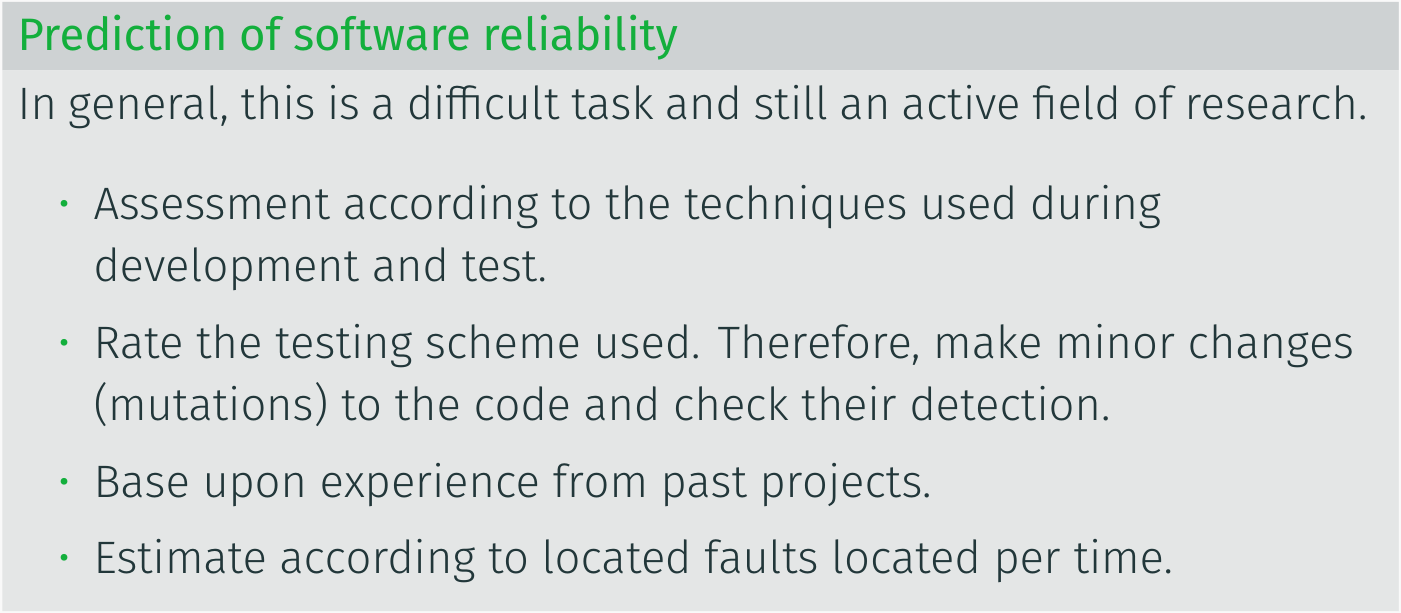
\includegraphics{images/safety/image-15.png}

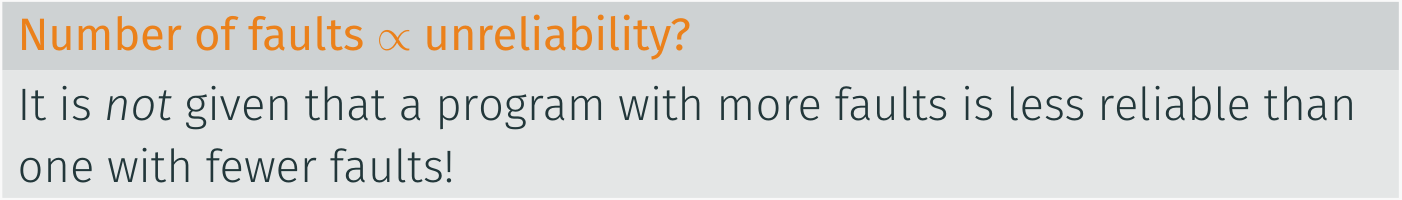
\includegraphics{images/safety/image-16.png}

\subsection{Reliability assessment}\label{reliability-assessment}

\textbf{Task}: demonstrate that a system meets its reliability
requirement.

\begin{tcolorbox}[enhanced jigsaw, toprule=.15mm, opacityback=0, colbacktitle=quarto-callout-tip-color!10!white, breakable, colframe=quarto-callout-tip-color-frame, title=\textcolor{quarto-callout-tip-color}{\faLightbulb}\hspace{0.5em}{How to\ldots{}}, left=2mm, arc=.35mm, toptitle=1mm, bottomrule=.15mm, rightrule=.15mm, titlerule=0mm, bottomtitle=1mm, leftrule=.75mm, opacitybacktitle=0.6, coltitle=black, colback=white]

\ldots{} proof that a system fails less then once in \(1\times 10^{9}\)
hour (i.e. \(\approx 100 000\) year) of operation?

{\textcolor{OliveGreen}{Trust the development techniques}}.

\end{tcolorbox}

\subsection{Software - Formal Methods}\label{software---formal-methods}

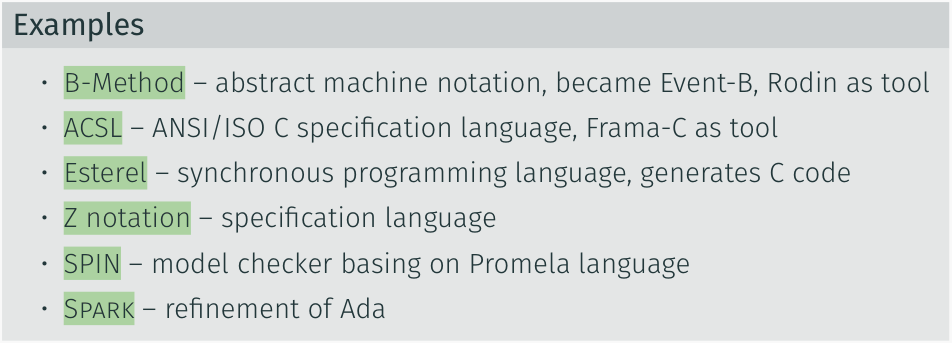
\includegraphics{images/safety/image-17.png}

\subsubsection{Spark}\label{spark}

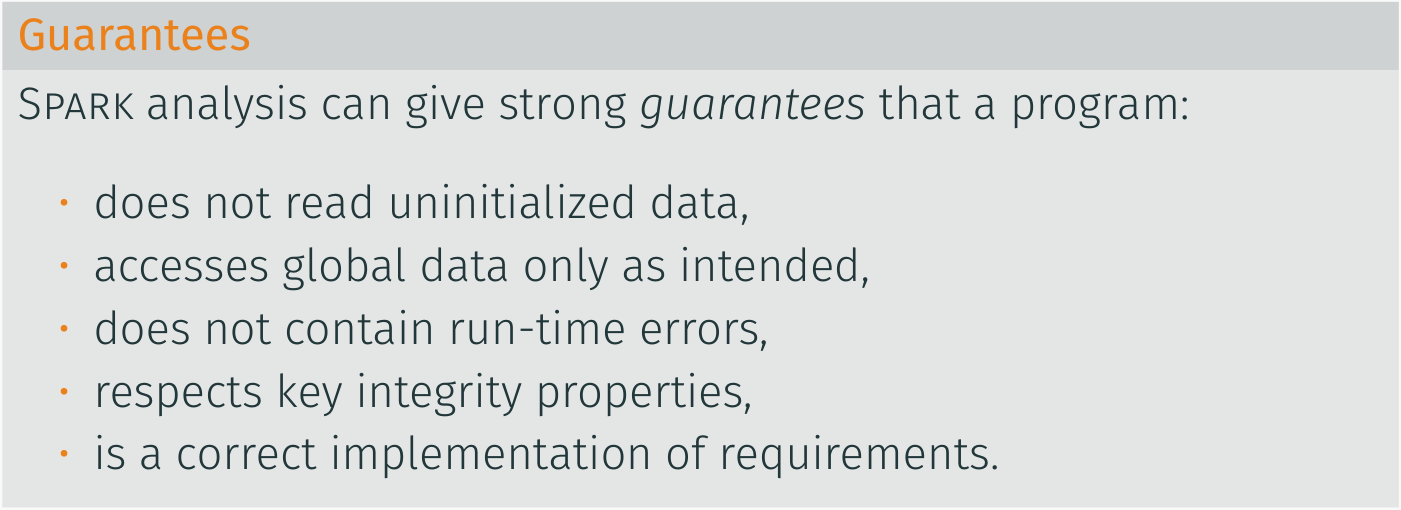
\includegraphics{images/safety/image-19.png}

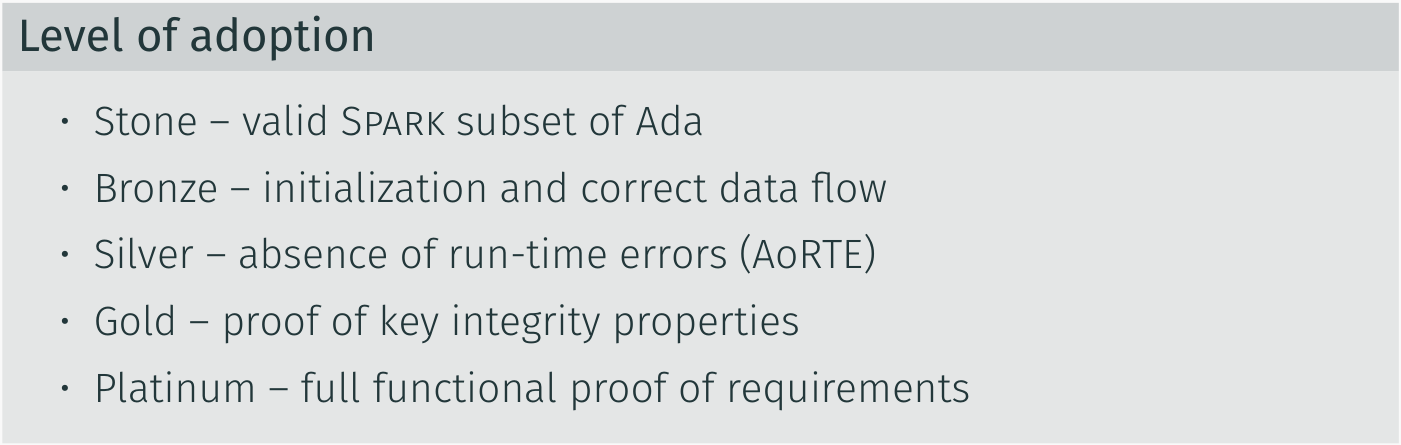
\includegraphics{images/safety/image-18.png}

\phantomsection\label{annotated-cell-43}%
\begin{Shaded}
\begin{Highlighting}[]
\KeywordTok{procedure} \DecValTok{Increment}\NormalTok{ (X }\OtherTok{:} \KeywordTok{in} \KeywordTok{out} \DataTypeTok{Integer}\NormalTok{)}
\KeywordTok{with}
\NormalTok{    Global =\textgreater{} }\KeywordTok{null}\NormalTok{, }\hspace*{\fill}\NormalTok{\circled{1}}
\NormalTok{    Depends =\textgreater{} (X }\OtherTok{=\textgreater{}}\NormalTok{ X), }\hspace*{\fill}\NormalTok{\circled{2}}
\NormalTok{    Pre =\textgreater{} X \textless{} Integer\textquotesingle{}Last, }\hspace*{\fill}\NormalTok{\circled{3}}
\NormalTok{    Post =\textgreater{} X = X\textquotesingle{}Old + 1 }\hspace*{\fill}\NormalTok{\circled{4}}
  \ControlFlowTok{is}
  \KeywordTok{begin}
\NormalTok{    X }\OtherTok{:=}\NormalTok{ X }\OtherTok{+} \DecValTok{1}\NormalTok{;}
  \KeywordTok{end Increment;}
\end{Highlighting}
\end{Shaded}

\begin{description}
\tightlist
\item[\circled{1}]
\textbf{Global}: does not read or write any global variables
\item[\circled{2}]
\textbf{Dependance}: Value of \textbf{X} after call depends on the
(previous) value of \textbf{X}
\item[\circled{3}]
\textbf{Condition}: \texttt{Increment} only callable if
\(X \leq \text{max value}\)
\item[\circled{4}]
\textbf{Conformance}: Check if the function does actually produce the
desired result.
\end{description}

\begin{tcolorbox}[enhanced jigsaw, toprule=.15mm, opacityback=0, colbacktitle=quarto-callout-caution-color!10!white, breakable, colframe=quarto-callout-caution-color-frame, title=\textcolor{quarto-callout-caution-color}{\faFire}\hspace{0.5em}{Vorsicht}, left=2mm, arc=.35mm, toptitle=1mm, bottomrule=.15mm, rightrule=.15mm, titlerule=0mm, bottomtitle=1mm, leftrule=.75mm, opacitybacktitle=0.6, coltitle=black, colback=white]

This check is done by \emph{Spark}, \textbf{NOT} \emph{Ada}.

These properties are not only declared, but these are \textbf{proved} by
a dedicated proof-engine \texttt{GNATprove}!

\end{tcolorbox}

\subsection{Hardware - Safety
Processors}\label{hardware---safety-processors}

\subsubsection{Hercules RM42 MCU}\label{hercules-rm42-mcu}

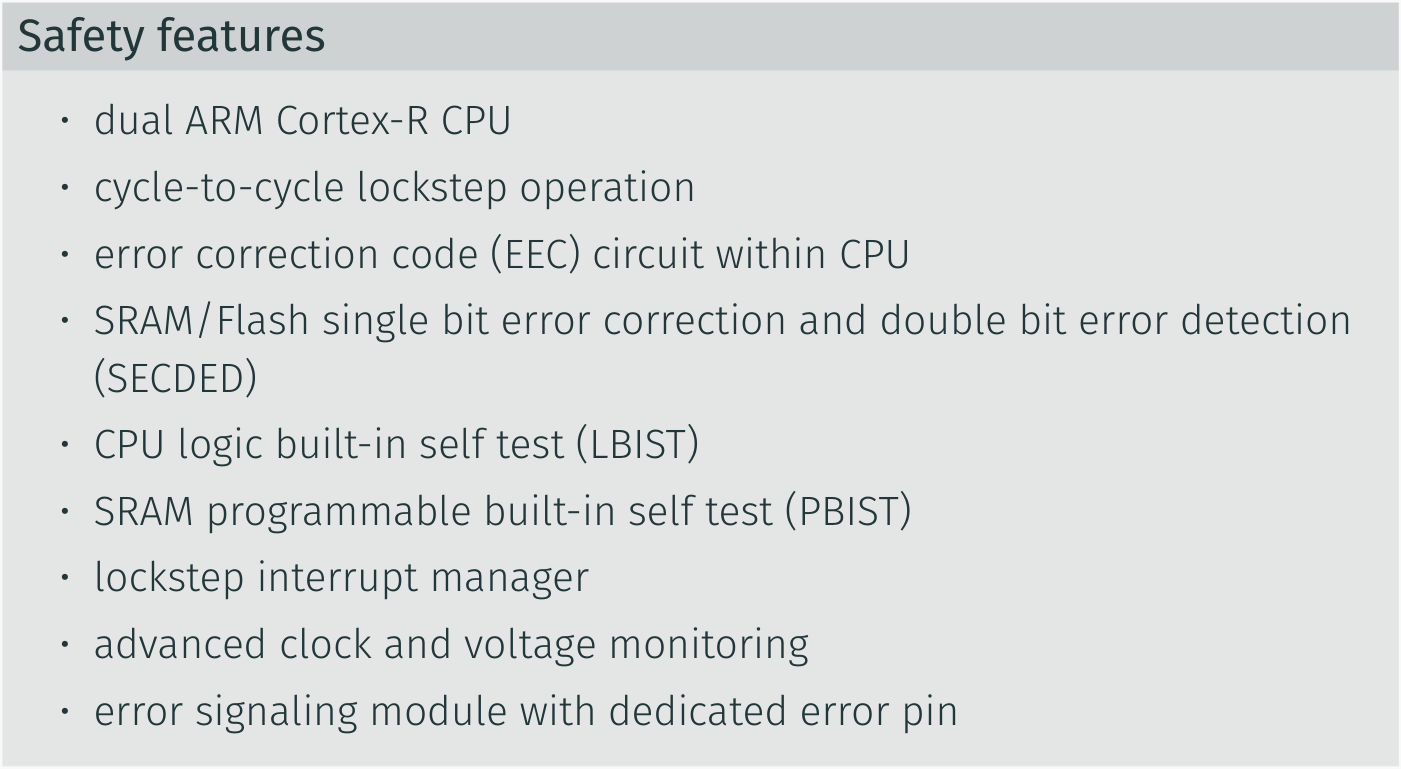
\includegraphics{images/safety/image-21.png}

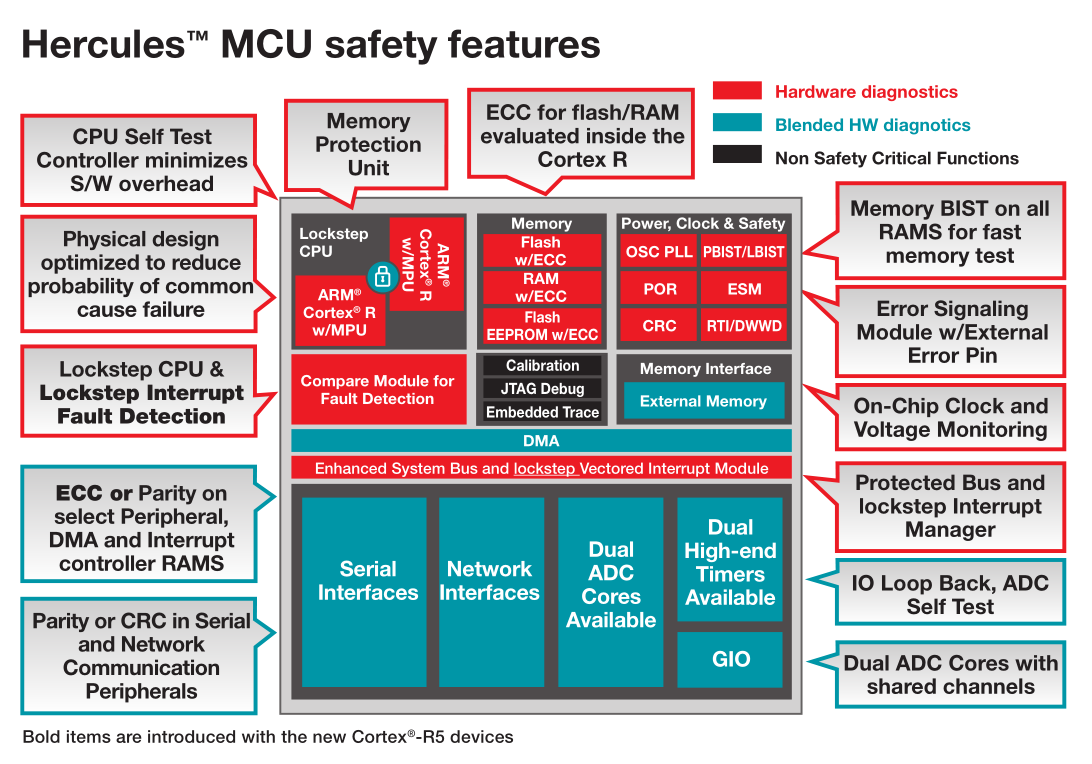
\includegraphics{images/safety/image-20.png}

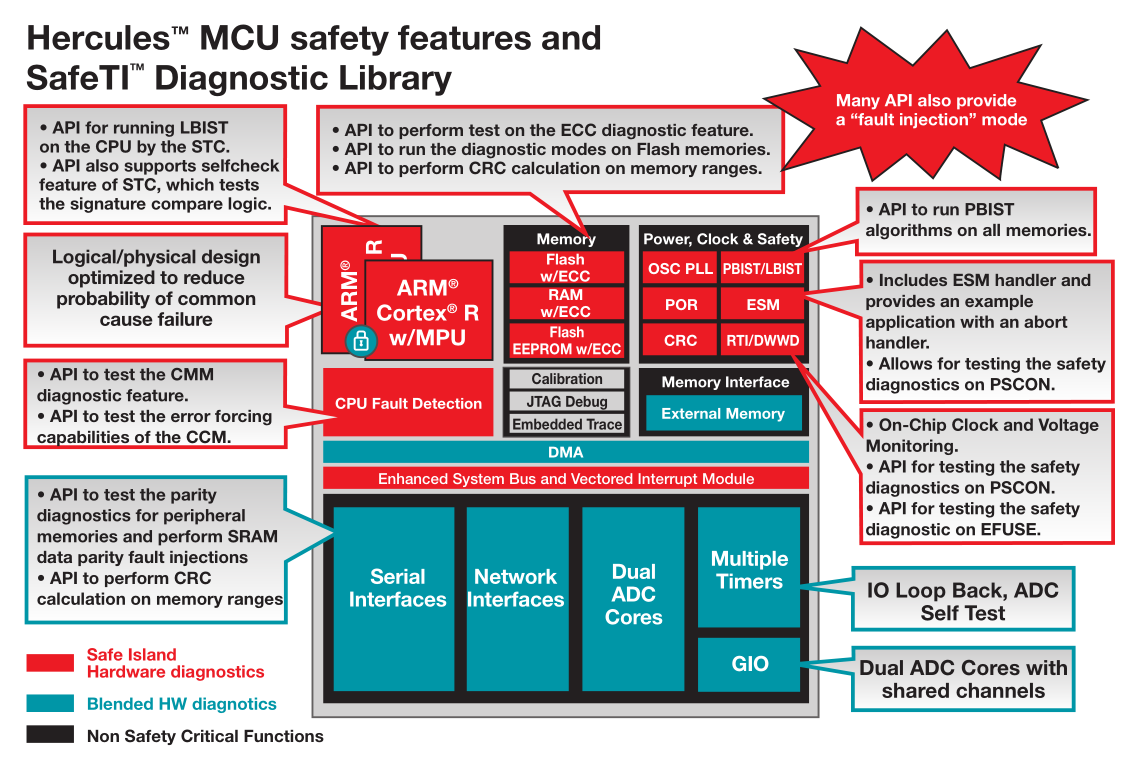
\includegraphics{images/safety/image-22.png}

\subsubsection{Dual CPU}\label{dual-cpu}

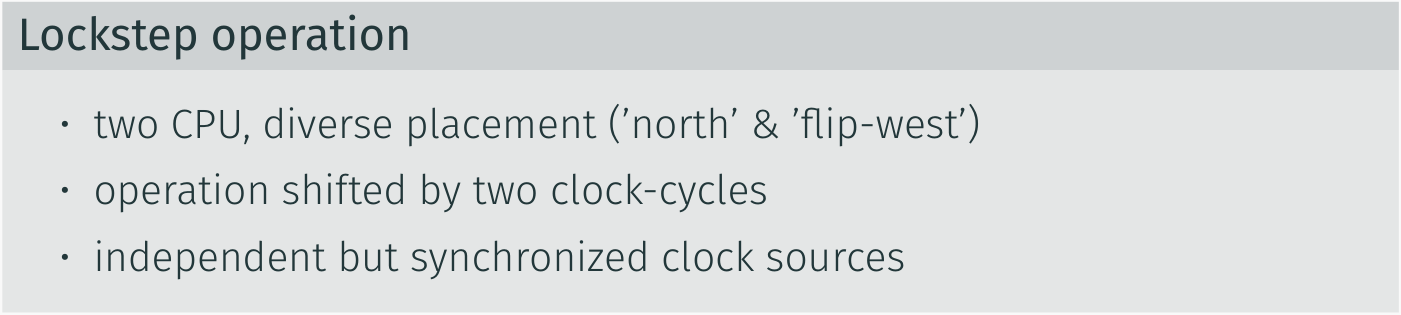
\includegraphics{images/safety/image-26.png}

\includegraphics{images/safety/image-23.png}

\subsubsection{Memory}\label{memory}

\includegraphics{images/safety/image-25.png}

\includegraphics{images/safety/image-24.png}

\subsubsection{Watchdog}\label{watchdog}

\includegraphics{images/safety/image-27.png}

\includegraphics{images/safety/image-28.png}

\newpage

\section{Trends - Low Power}\label{trends---low-power}

\begin{center}
\includegraphics[width=7cm,height=\textheight]{images/trends_meme.jpg}
\end{center}

\subsection{Firm-/Software
Optimierungen}\label{firm-software-optimierungen}

\begin{itemize}
\tightlist
\item
  \texttt{float} \& \texttt{double} vermeiden \(\rightarrow\) sehr
  Rechenintensiv bei Systemen ohne FPU (und auch sonst)
\item
  Divisionen sind rechenintensiv, ausser durch Zweierpotenzen
  \(2,4,8,16,...\), wo Bitshifting gemacht wird.
\item
  Optimierungen einschalten beim Kompilieren :-)
\end{itemize}

\newpage

\section{Anhang}\label{anhang}

\subsection{Crypto}\label{crypto-1}

\subsubsection{Permutation Tabellen}\label{permutation-tabellen}

\begin{center}
\includegraphics{images/crypto/permutation tables.pdf}
\end{center}



\end{document}
